%My thesis!
%\documentclass[11pt,a4paper,titlepage]{report}
\documentclass[a4paper,11pt,openright,twoside]{book}
\usepackage{amsmath}
\usepackage{ amssymb }
\usepackage{calligra}
\usepackage{amsfonts}
\usepackage[english]{babel}
\usepackage{verbatim}
\usepackage{indentfirst}
\usepackage{fancyhdr}
\usepackage{amsthm}
\usepackage{graphicx}
\usepackage{indentfirst}
\usepackage{microtype}
\usepackage{lmodern}
\usepackage{braket}
\usepackage{todonotes}

\usepackage[font=small,labelfont=bf]{caption}  %per la didascalia delle immagini
\usepackage{mathrsfs}  %per fare le lettere calligrafiche
\usepackage{bm}  %per mettere le lettere greche in grassetto
\usepackage[T1]{fontenc}     %pacchetto lettere accentate
\usepackage[utf8]{inputenc}   %pacchetto lettere accentate

\newtheorem*{remark}{Remark}

\newcommand{\HRule}{\rule{\linewidth}{0.5mm}}

% MER says: You can have no-indent later if you want to, but not while
% I'm reading this.
%\setlength\parindent{0pt} % toglie identazione ovunque
\usepackage[sc]{mathpazo}
\usepackage{tikz}

\newcommand{\mesh}{\mathcal{T}_t}

% -----------------

\begin{document}

%--------------------------

\begin{titlepage}
%\begin{adjustwidth*}{10pt}{-40pt}
\begin{center}
\vspace*{-2.7cm}

\includegraphics{images/aquila_nome}
\\
\rule{\textwidth}{1pt}
\\[0.5cm]
{\Large DEPARTMENT OF MATHEMATICS}
\\[0.35cm]
{\Large MASTER DEGREE IN MATHEMATICS}
\\[3.5cm]
\textsc{\huge \textbf{Simulating CSF flow in an idealized geometry of the subarachnoid space}}
%\\[0.4cm]
%{\Large March 25th, 2015}
%\\[3cm]
\\[4cm]
\begin{minipage}{0.5\textwidth}
\flushleft {
\large Advisors: \\
 \textbf{Prof. Eleuterio F. Toro} \rule{0pt}{2.5ex}\\
 \normalsize University of Trento\\[0.4cm]
\large \textbf{Dr. Marie E. Rognes} \\
\large \textbf{Ms. Eleonora Piersanti} \\
\large \textbf{Dr. Victor Haughton} \\
 \normalsize Simula Research Laboratory\\[0.4cm] \rule{0pt}{2.5ex}}\\
\end{minipage}
\begin{minipage}{0.45\textwidth}
\vspace{-3.2cm}
\flushright {\large
Student: \\
\rule{0pt}{2.5ex} \textbf{Carlo Cisale}\\
\normalsize University of Trento} \\
\end{minipage}

\vspace*{\fill}
{\textsc{\normalsize October $25^{th}, 2017$}}
\rule{\textwidth}{1pt}


\end{center}
%\end{adjustwidth*}
\newpage
\thispagestyle{empty}
\phantom{}
\end{titlepage}
\newpage
\thispagestyle{empty}

\pagenumbering{roman}
\chapter*{\LARGE Acknowledgments}
jyfufuyhfh
jhgcghk
jgchgc
gchghgcgh

\newpage

{\Large \textbf{List of acronyms}}



%--------------------------
\newpage
\tableofcontents


\newpage
\pagenumbering{arabic}

\chapter{Introduction}
% wiki
% article martin, kalata, loth,...

The brain and the spinal cord are surrounded by the cerebrospinal fluid (CSF), a clear fluid that has almost same viscosity as water and, in an healthy person, is composed of dilute amounts of proteins and monoamines. It provides nutrients and remove waste from the brain, and acts as a cushion for the brain, providing damping between the brain and the skull when sudden movements of the cranium occur. The CSF moves in a pulsatile way through the subarachnoid space (SAS), a space between the arachnoid mater and the pia mater. The CSF flow is passive and its pulsatile nature has been associated with changes in blood volume within the cranial cavity due to the cardiac cycle [reference].

\chapter{Medical background}

\chapter{Mathematical models}

\section{The Navier-Stokes equations on a fixed domain}

% References:
% - Quarteroni
% - Vegard
% - Drosdal

The flow in the SAS and in the spinal cord can be described by the incompressible Navier-Stokes equations for Newtonian fluids. They describe the motion of a fluid with constant density $\rho$ in a domain $\Omega \subset \mathbb{R}^d$ (where $d=2,3$). They read

\begin{align}
\label{eq:ns:0}
\rho \dot{\mathbf{u}}
+ \rho \nabla \mathbf{u} \cdot \mathbf{u}
- \nabla \cdot \sigma(\mathbf{u},p)
&= \mathbf{f},  && \mathbf{x} \in \Omega, \, t>0 \\
\nabla \cdot \mathbf{u} &= 0, && \mathbf{x} \in \Omega, \, t>0
\end{align}

We are going to solve the problem for the velocity field $\mathbf{u}(\mathbf{x},t)$, and the pressure field $p(\mathbf{x},t)$, where $\mathbf{x} = (x,y)$. The quantity $\sigma(\mathbf{u}, p)$, is the Cauchy stress tensor for a Newtonian fluid, given by

\begin{equation}
\sigma(\mathbf{u}, p) = \mu \nabla \mathbf{u} - p \mathbb{I}.
\end{equation}

The constant $\mu$ represents the fluid viscosity, while $\mathbf{f}$ denotes a forcing term per unit of mass. Substituting $\sigma$ in~\eqref{eq:ns:0} we obtain

\begin{align}
\rho \dot{\mathbf{u}} + \rho \nabla \mathbf{u} \cdot \mathbf{u} - \nabla \cdot (\mu \nabla \mathbf{u} - p \mathbb{I}) &= \mathbf{f}.
\end{align}

Since $\mu$ is constant, we have

\begin{align}
\label{eq:ns:3}
\rho \dot{\mathbf{u}} + \rho \nabla \mathbf{u} \cdot \mathbf{u} - \mu \Delta \mathbf{u} +  \nabla p &= \mathbf{f}, \\
\label{eq:ns:3bis}
\nabla \cdot \mathbf{u} &= 0.
\end{align}

The term $(\mathbf{u} \cdot \nabla)\mathbf{u}$ describes the process of convective transport (	QUARTERONI). ~\cite{}.\\
In order for the problem to be well posed, it is necessary to assign an initial condition

\begin{equation}
\mathbf{u} (\mathbf{x}, 0) = \mathbf{u}_0(\mathbf{x}) \quad \forall \mathbf{x} \in \Omega,
\end{equation}

where $\mathbf{u}_0$ is a given divergence-free vector field, together with suitable boundary conditions, such as

\begin{align}
\mathbf{u}(\mathbf{x},t) &= \phi (\mathbf{x}, t) & \forall \mathbf{x} \in \Gamma_D \\
\label{eq:ns:8}
\left( \mu \frac{\partial \mathbf{u}}{\partial \mathbf{n}} - p\mathbf{n} \right) (\mathbf{x},t) &= \psi(\mathbf{x},t) & \forall \mathbf{x} \in \Gamma_N
\end{align}


where $\phi$ and $\psi$ are given vector functions, while $\Gamma_D$ and $\Gamma_N$ give a partition of the domain boundary $\partial \Omega$, that is $\Gamma_D 	\cup \Gamma_N = \partial \Omega, \mathring{\Gamma}_D \cap \mathring{\Gamma}_N = \emptyset$. Moreover, $\mathbf{n}$ is the outward unit normal vector to $\partial \Omega$. Equation (\ref{eq:ns:8}) can also be written in another form

\begin{equation}
\sigma \cdot \mathbf{n} = \psi(\mathbf{x}, t)  \quad \forall \mathbf{x} \in \Gamma_N.
\end{equation}

\begin{remark}
\normalfont{In our notation, if $\mathbf{u} = (u_x, u_y)^T$ and $\mathbf{x} = (x, y)^T$, then $\nabla \mathbf{u}$ is defined as

\[
\nabla \mathbf{u} =
\begin{pmatrix}
\frac{\partial u_x}{\partial x} & \frac{\partial u_x}{\partial y} \\
\frac{\partial u_y}{\partial x} & \frac{\partial u_y}{\partial y}
\end{pmatrix}
\]


}
\end{remark}


\section{Navier-Stokes on a moving domain}
% From Donea, Duarte, Vegard

Numerical simulation of two-dimensional viscous incompressible fluid with free boundaries is getting a lot of attention in the past decades for the several applications in industry and medicine. An important consideration when coding problems in this class is the use of an appropriate \emph{kinematical description} of the continuum. Such a choice determines the relationship between the deforming continuum and the finite mesh of the computing zones, and the ability of the numerical method to deal with large distortions. \\
The algorithm of continuum mechanics usually make use of two classical descriptions of motion: the \emph{Lagrangian} description and the \emph{Eulerian} description. The arbitrary Lagrangian-Eulerian description (or ALE) has the advantage to combine the classical kinematical descriptions, while reducing their drawbacks [Donea, Duarte, Vegard]. \\
In Lagrangian algorithms, each individual node of the computational mesh follows the associated material particle during motion, and they are mostly used in structural mechanics.
In Eulerian algorithms the computational mesh is fixed and the continuum moves with the respect to the grid. These algorithms are widely used in fluid dynamics problems.
In order to combine the best features of both algorithms, the ALE description was developed. We are going to talk about it later. Now let us focus on the classical descriptions of motion.


\subsection{Lagrangian and Eulerian descriptions of motion}
Let us consider a domain $\Omega_{\mathbf{X}} \in \mathbb{R}^3$ consisting of material particles $\mathbf{X}$. The domain can undergo deformations, and the deformed domain $\Omega_\mathbf{x}$ is the current configuration at time $t$.

\todo[inline]{Put image from Vegard}

We define one-to-one mapping:

\todo[inline]{Put mapping}

which takes any point $\mathbf{X}$ in the reference configuration to a new position $\mathbf{x} = \beta(\mathbf{X},t)$ at time $t$. As the mapping is one-to-one, it is also possible to keep track of the history of the motion by the inverse $\beta^{-1}$. Time is measured with the same variable $t$ in both domains. The gradient of $\beta$ with respect to $(\mathbf{X},t)$ can be written in the matrix forms as

\begin{equation}
\frac{\partial \beta}{\partial(\mathbf{X}, t)} = 
\begin{pmatrix}
\frac{\partial \mathbf{x}}{\partial \mathbf{X}} & \mathbf{v} \\
\mathbf{0}^T & 1
\end{pmatrix}
\end{equation}

where the material velocity

\begin{equation}
\mathbf{v}(\mathbf{X}, t) = \frac{\partial \mathbf{x}}{\partial t}|_\mathbf{x},
\end{equation}

is the temporal change in the spatial variable $\mathbf{x}$ while holding $\mathbf{X}$ fixed, while $\mathbf{0}^T$ denotes a null vector. \\
In the Lagrangian description all the quantities are expressed in terms of the reference configuration $\Omega_{\mathbf{X}}$ and time, i.e. even though the material is deformed, we can still compute displacements and particle velocities using the material coordinates $\mathbf{X}$.
Since the grid coincides with the material coordinates, there are no convective term in the Lagrangian description, and it coincides with a moving control volume consisting of the same material points at all time. When a material undergoes large deformations, or for instance vortices or turbulences occur, the material velocity becomes difficult to handle in the Lagrangian approach.

In fluid mechanics, the \emph{Eulerian} approach describes the flow of a fluid through a fixed region in space and in each point we can measures its properties and quantities, such as velocity, pressure, temperature. The conservation equations in the Eulerian description are expressed in terms of the spatial coordinates $\mathbf{x}$ and time, and are neither connected to a reference configuration nor the material coordinates. Hence, large deformations are not an issue, since the material can enter and leave the fixed domain. The movement of a material through a fixed region results in convective effects, and convective operators can often be problematic in computational fluid dynamics since they are not symmetric.


\subsection{The Arbitrary-Eulerian Lagrangian formulation}
The ALE formulation is common is fluid-structure interaction problems and it provides a referential system which is neither attached to the material points nor totally fixed in space, i.e. the nodes of the computational mesh may be moved with the continuum in normal Lagrangian fashion, or be held fixed in Eulerian manner, or be moved in some arbitrarily specified way.

The following derivation is taken from [Donea, Vegard].

Since we need a new set of coordinates, an independent referential system with reference coordinates $\chi$ is introduced. Hence, we have two new mappings to relate all the configurations as shown in the picture below.

\todo[inline]{Put picture of mapping of the 3 from Vegard}

The mappings are defined similarly to $\beta$:

\todo[inline]{Put mapping}

and the gradient of $\gamma$ is 

\begin{equation}
\frac{\partial \gamma}{\partial(\chi, t)} = 
\begin{pmatrix}
\frac{\partial \mathbf{x}}{\partial \chi} & \mathbf{w} \\
\mathbf{0}^T & 1
\end{pmatrix}
\end{equation}

where we define $\mathbf{w}$ as the mesh velocity, i.e.

\begin{equation}
\mathbf{w}(\chi, t) = \frac{\partial \mathbf{X}}{\partial t}|_\chi,
\end{equation}

Hence, the fluid moves with velocity $\mathbf{v}$ and the domain moves with velocity $\mathbf{w}$.

To complete the relation between the different velocities, we define the inverse of $\alpha$ as

\todo[inline]{Put mapping}

Its gradient is given by

\begin{equation}
\frac{\partial \alpha^{-1}}{\partial(\mathbf{X}, t)} = 
\begin{pmatrix}
\frac{\partial \chi}{\partial \mathbf{X}} & \hat{\mathbf{v}}\\
\mathbf{0}^T & 1
\end{pmatrix}
\end{equation}

where the velocity

\begin{equation}
\label{eq:ale:4}
\hat{\mathbf{v}} (\mathbf{X},t) = \frac{\partial \chi}{\partial t}_{|_{\mathbf{X}}}
\end{equation}

denotes the temporal change in the reference system while keeping the material particle $\mathbf{X}$ fixed. Therefore, the velocity $\mathbf{\hat{v}}$ can be interpreted as the particle velocity in the referential domain.

Since $\beta = \alpha \cdot \alpha^{-1} = \gamma(\alpha^{-1}(\mathbf{X},t))$ and obtain a relation between the different velocities by differentiating $\beta$:

\begin{align*}
\frac{\partial \beta}{\partial (\mathbf{X},t)} (\mathbf{X},t)
& = \frac{\gamma}{\partial (\chi, t)}(\alpha^{-1}(\mathbf{X},t)) \frac{\partial \alpha^{-1}}{\partial(\mathbf{X},t)}(\mathbf{X},t) \\
& = \frac{\partial \gamma}{\partial (\chi, t)}(\chi,t)) \frac{\partial \alpha^{-1}}{\partial(\mathbf{X},t)}(\mathbf{X},t).
\end{align*}

In matrix form, the previous equation reads

\begin{equation}
\begin{pmatrix}
\frac{\partial \mathbf{x}}{\partial \mathbf{X}} & \mathbf{v}\\
\mathbf{0}^T & 1
\end{pmatrix} = 
\begin{pmatrix}
\frac{\partial \mathbf{x}}{\partial \chi} & \mathbf{w}\\
\mathbf{0}^T & 1
\end{pmatrix}
\begin{pmatrix}
\frac{\partial \chi}{\partial \mathbf{X}} & \hat{\mathbf{v}}\\
\mathbf{0}^T & 1
\end{pmatrix}
\end{equation}

Multiplying the matrices on the right hand side, we obtain the following equation

\begin{equation}
\mathbf{v} = \frac{\partial \mathbf{x}}{\partial \chi} \cdot \hat{\mathbf{v}} + \mathbf{w}
\end{equation}

that relates the different velocities. We define the \emph{convective velocity} as

\begin{equation}
\mathbf{c} := \mathbf{v-w} = \frac{\partial \mathbf{x}}{\partial \chi} \cdot \hat{\mathbf{v}}
\end{equation}

which is the relative velocity between the material and the mesh.

In order to obtain relations between quantities to formulate the balance equations, let us define the scalar quantity $Q$ defines as $Q^{*}(\mathbf{x},t)$, $Q(\chi,t)$, and $Q^{**}(\mathbf{X},t)$ in the spatial, reference, and material domain respectively.
To obtain a relation between the spatial description $Q$, and the material description $Q^{**}$ we use the previous the mapping $\beta$ that we have previously used:

\begin{equation}
Q^{**}(\mathbf{X},t) = Q(\beta(\mathbf{X},t),t) = Q \cdot \beta.
\end{equation}

The gradient of $Q^{**}$ can then be computed as

\begin{equation}
\label{eq:ale:1}
\frac{\partial Q^{**}}{\partial (\mathbf{X}, t)} (\mathbf{X},t) = 
\frac{\partial Q}{\partial (\mathbf{x}, t)} (\mathbf{x},t)
\frac{\partial \beta}{\partial (\mathbf{X}, t)} (\mathbf{X},t),
\end{equation}

or in the matrix form

\begin{equation}
\label{eq:ale:2}
\begin{pmatrix}
\frac{\partial Q^{**}}{\partial \mathbf{X}} & \frac{\partial Q^{**}}{\partial t}
\end{pmatrix} = 
\begin{pmatrix}
\frac{\partial Q}{\partial \mathbf{x}} & \frac{\partial Q}{\partial t}
\end{pmatrix}
\begin{pmatrix}
\frac{\partial \mathbf{x}}{\partial \mathbf{X}} & \mathbf{v}\\
\mathbf{0}^T & 1
\end{pmatrix} 
\end{equation}

Multiplying the matrices, we bbtain the equation that relates material and spatial derivatives:

\begin{equation}
\label{eq:ale:3}
\frac{\partial Q^{**}}{\partial t} = \frac{\partial Q}{\partial t}
+ \frac{\partial Q}{\partial \mathbf{x}} \cdot \mathbf{v}
\end{equation}

To ease notation we now recognize the material and spatial time derivatives $\frac{\partial Q^{**}}{\partial t} = \frac{\partial Q}{\partial t}_{|_\mathbf{X}}, \,  \frac{\partial Q}{\partial t} = \frac{\partial Q}{\partial t}_{|_\mathbf{x}}$, and define the material and spatial derivatives in the following way

\begin{equation}
\frac{d}{dt} := 	\frac{\partial}{\partial t}_{|_\mathbf{X}} \qquad
\frac{\partial}{\partial t} := \frac{\partial}{\partial t}_{|_\mathbf{x}}
\end{equation}

Now we can rewrite the relation (\ref{eq:ale:3}) can be written in the form

\begin{equation}
\label{eq:ale:6}
\frac{d Q}{d t} = \frac{\partial Q}{\partial t} + (\mathbf{v} \cdot \nabla) Q.
\end{equation}

The next step is to relate the material and the reference description, respectively $Q^{**} and Q^{*}$, by the mapping $\alpha$. This relation is the following

\begin{equation}
Q^{**} = Q^{*} \cdot \alpha^{-1}.
\end{equation}

By proceeding as in (\ref{eq:ale:1})-(\ref{eq:ale:2}), we obtain the relation between material and reference time derivatives:

\begin{equation}
\label{eq:ale:3}
\frac{\partial Q^{**}}{\partial t} = \frac{\partial Q^{*}}{\partial t}
+ \frac{\partial Q}{\partial \chi} \cdot \hat{\mathbf{v}}.
\end{equation}

To express the spatial derivative of $Q^{*}$ in the spatial domain, we use the definition of $\hat{\mathbf{v}}$ from equation (\ref{eq:ale:4}) and obtain

\begin{equation}
\frac{\partial Q^{**}}{\partial t} = \frac{\partial Q^{*}}{\partial t}
+ \frac{\partial Q}{\partial \mathbf{x}} \cdot \mathbf{c}.
\end{equation}

This equation can be rewritten in the more common notation

\begin{equation}
\label{eq:ale:5}
\frac{d Q}{d t} = \frac{\partial Q}{\partial t}_{|_\chi} + (\mathbf{c} \cdot \nabla) Q
\end{equation}

and it is called the \emph{fundamental ALE equation}, which states that the time derivative in the material configuration is equal to its local (reference) derivative plus a convective term, taking into account the relative difference in velocity between the two systems. These relations also hold for vector quantities.

By combining equations (\ref{eq:ale:5})-(\ref{eq:ale:6}) we have

\begin{equation}
\label{eq:ale:7}
\frac{\partial Q}{\partial t} = \frac{\partial Q}{\partial t}_{|_\chi} - (\mathbf{w} \cdot \nabla) Q.
\end{equation}

which relates the spatial time derivative to the reference time derivative.

The momentum equation [PUT SOME REFERENCE FOR DERIVATION OF NAVIER STOKES] can be written in terms of the material derivatives as

\begin{equation}
\rho \frac{d \mathbf{v}}{d t} = \rho (\frac{\partial \mathbf{v}}{\partial t} + (\mathbf{v} \cdot \nabla)\mathbf{v}) = \nabla \cdot \sigma
\end{equation}

Using equation (\ref{eq:ale:7}), the spatial time derivatives can be replaced to obtain its ALE formulation

\begin{equation}
\rho (\frac{\partial \mathbf{v}}{\partial t}_{|_\chi} + (\mathbf{c} \cdot \nabla)\mathbf{v}) = \nabla \cdot \sigma. 
\end{equation}

The previous equation holds in \emph{any} time-dependent domain which does not necessarily need to coincide with the movement of material particles. The latter also shows that in order to obtain the ALE formulation of the momentum equation from the Eulerian formulation is to replace the convective velocity with the relative velocity between the material and the mesh.


\section{Modelling the idealized geometry of the SAS}
We now want to model the flow of cerebrospinal fluid in the subarachnoid space, using the previous informations. In the first section, we will use Navier-Stokes equation in a fixed domain, while in the second one we will use the ALE formulation of Navier-Stokes equations. Since CSF consists of $99 \% $ of water [REFERENCE], it is modeled as water at $37 \deg C$, i.e. the fluid density will be $\rho = 10^{-3} \frac{g}{mm^3}$, while the fluid viscosity is $\mu = 0.700 \frac{mm^2}{s}$. 


\subsection{Fixed boundary}
Let us consider a two-dimensional rectangular (fixed) domain $\Omega^0 = [0, 2]
\times [0, 60]$, representing the right portion of the subarachnoid space, between the spinal cord and the surrounding tissue from C1 to C7 vertebrae, approximately. We define the
\begin{itemize}
\item
  top boundary: $\partial \Omega_{\rm top}^0 = \{ (x, y) | y = 60\}$;
\item
  bottom boundary: $\partial \Omega_{\rm bottom}^0 = \{ (x, y) | y = 0\}$;
\item
  tissue boundary: $\partial \Omega_{\rm tissue}^0 = \{ (x, y) | x = 2\}$;
\item
  cord boundary: $\partial \Omega_{\rm cord}^0 = \{ (x, y) | x = 0\}$;
\end{itemize}
and thus $\partial \Omega^0 = \partial \Omega_{\rm top}^0 \cup
\partial \Omega_{\rm bottom}^0 \cup \partial \Omega_{\rm cord}^0 \cup
\partial \Omega_{\rm tissue}^0$.

\begin{figure}

\todo[inline]{put two images: left spinal cord. right: rectangle with boundary labels.}

  \caption{Left: spinal cord in the SAS. Right: Schematic illustration
    of computational domain}
\end{figure}

We set the following boundary condition on $\partial \Omega^0$: on the boundaries $\partial \Omega_{\rm cord}^0$ and $\partial \Omega_{\rm tissue}^0$ we set the so called \emph{no-slip condition} $\mathbf{u = 0}$, i.e. the fluid velocity on those boundaries is zero. This condition does not allow the fluid to flow through the boundaries.
In order to simulate an oscillatory fluid flow, we set a pressure difference on the top and bottom boundaries, as follows:

\begin{align}
\label{eq:bc:6}
\sigma \cdot \mathbf{n} &= \mu \frac{\partial \mathbf{u}}{\partial \mathbf{n}} - p \mathbf{n} = -\bar{p} \mathbf{n} && \text { on } \partial \Omega_{\rm top}^0 \\
\label{eq:bc:6bis}
\sigma \cdot \mathbf{n} &= \mu \frac{\partial \mathbf{u}}{\partial \mathbf{n}} - p \mathbf{n} = \mathbf{0}  && \text { on } \partial \Omega_{\rm bottom}^0.
\end{align}

where $\bar{p}(t) = A \cdot sin(2\pi t)$ is a prescribed pressure, and $A = 9kPa$. We assume a heart rate of $60$ heart-beats per minute, so that the duration of the cardiac cycle is set to $1s$. During \textit{systole}, as blood flows into the brain, CSF flows down the Aqueduct of Sylvius. During \textit{diastole}, the opposite occurs. The sine term is added to reproduce the pulsatile motion of the fluid. 

\begin{figure}

\todo[inline]{put the rectangle with the corresponding boundary conditions.}

  \caption{Boundary conditions applied on $\partial \Omega^0$}
\end{figure}


\subsection{Moving boundary}
Our next step is to allow the domain and its boundary to move, and
solve the Navier-Stokes equations on this deforming domain. Let $\Omega^t$ denote the fluid domain which depends on time $t$, and
$\Omega^0$ denote the fixed fluid domain at $t = 0$. In
fluid-structure interaction, the fluid domain $\Omega^t$ consists of
the same material particles at all times, and moves with the material
points within the structure. Also assume that we have a mesh $\mesh$
of the domain $\Omega^t$. Let $\mathbf{w}$ denote the \emph{mesh velocity}.
  
%and $\mathbf{y}$ the \emph{mesh displacement} with respect to the reference domain $\Omega^0$, and thus by definition $\dot{\mathbf{y}} = \mathbf{w}$ where the superposed dot denotes the time derivative. 

%The movement of the domain $\Omega^t$ is governed by the mesh
%displacement, i.e.~for all $x(t) \in \Omega^t$, each corresponding to
%a point $\mathbf{X}_0 \in \Omega^0$, we have that
%\begin{equation}
%  \mathbf{X}(t) = \mathbf{X}_0 + \mathbf{y}(t)(X_0).
%\end{equation}
%\todo[inline]{Check the precise formulation carefully in Donea
%  reference e.g.}

An ALE formulation of the Navier-Stokes equations on the deforming
domain $\Omega^t$ reads: find the velocity $\mathbf{u}$ and the
pressure $p$ such that
\begin{align}
  \label{eq:ns:1}
  \rho \dot{\mathbf{u}}
  + \rho \nabla \mathbf{u} \cdot (\mathbf{u} - \mathbf{w})
  - \mu \Delta \mathbf{u} + \nabla p
  &= \mathbf{f},  & \text{in } \Omega^t, \\
  \label{eq:ns:2}
  \nabla \cdot \mathbf{u} &= 0, & \text{in } \Omega^t,
\end{align}
for $t \in (0, T]$, where $T=15$ is the final time (and the number of cardiac cycles of our simulations, that we need in order for the flow to fully develop). The quantity $\mathbf{f}$ is a given body force.
We will let the fluid domain boundary follow the changes on the
fluid-structure interface. Moreover, to move the entire domain, we
will use a \emph{Laplacian smoothing}
algorithm~\cite{Winslow1963}. More precisely, our mesh smoothing
equation reads: given some boundary velocity $\mathbf{w}_0$, find
$\mathbf{w}$ that satisfies
\begin{align}
\label{eq:bc:2}
- \Delta \mathbf{w} &= 0 	&& \text{in } \Omega^t, \\
\mathbf{w} &= \mathbf{w}_0 && \text{on } \partial \Omega^t .
\end{align}
\\
for each $t \in [0, T]$.


%Further,
%\begin{equation}
%  \partial \Omega^t_{\rm i} = \partial \Omega^0_{\rm i} + \mathbf{y}(t)(\partial \Omega^0_{\rm i}),
%\end{equation}
%for each $i$.

As what concerns the boundary conditions for the velocity $\mathbf{u}$, they remain the same also in the moving domain.
Now we have also to specify boundary conditions for the mesh velocity. We are interested in studying the effect of craniovertebral
decompression on the fluid flow and pressure dynamics in the
subarachnoid space. In particular, we assume that craniovertebral
decompression induces a change in the compliance of the tissue
surrounding the spinal canal~\cite{}. For simplicity, we aim to model
the compliance of the surrounding tissue via a boundary condition for
the fluid flow. 

For the mesh equation, we let the mesh velocity follow a gaussian profile on the tissue boundary, while the mesh velocity is assumed to
be zero (i.e.~the mesh boundary is fixed) on the remaining boundary:
\begin{align}
\label{eq:bc:5}
\mathbf{w} &= \bar{\mathbf{w}}  \qquad \text{ on } \partial \Omega_{\rm tissue}^t,\\
\mathbf{w} &= \mathbf{0}  \qquad \text{ on } \partial \Omega^t \setminus \partial \Omega_{\rm tissue}^t
\end{align}

where $\bar{\mathbf{w}} = (B \cdot sin(4\pi t) \cdot \frac{1}{\sqrt{2 \pi s^2}} \, e^{- \frac{1}{2} \, \frac{(y - m)^2}{s^2}}  , 0)$, and $s = 3$ and $m = 6$ are respectively the variance and the mean value of the gaussian function. We multiplied the gaussian function by a sine in order to simulate oscillatory movement of the mesh, and the quantity $B$ is the amplitude of the movement. In our simulations we will use different amplitudes of the movement, in order to compare quantities to understand if the movement of the mesh plays a role in the CSF flow.

\begin{figure}

\todo[inline]{put the rectangle with the corresponding boundary conditions for the mesh velocity}

\end{figure}


In order to simplify the notation, in the following sections we are going to drop the $t$ when we talk about a moving boundary (e.g. $\partial \Omega^t$ will simply be $\partial \Omega$).

%Moreover, note that $\partial \Omega_{\rm cord}$ and $\partial \Omega_{\rm tissue}$ are \textit{physical} boundaries, i.e.~they model portions of the spinal cord and surrounding tissue. This means that $\mathbf{u}$ and $\mathbf{w}$ should have the same value on these boundaries, since the fluid follows the movement (if any) of the walls.



\chapter{Numerical methods}

\section{Finite element formulation}

\section{Weak formulation of N-S on fixed domain}

In order to obtain the weak formulation of the system~\eqref{eq:ns:3}--~\eqref{eq:ns:3bis}, we multiply the first equation by a test function $\mathbf{v}$ in a space $\hat{V}$ to be specified, and the second equation by a test function $q$ in a space $Q$, and integrate over $\Omega$. 
We obtain:

\begin{align}
\label{eq:ns:9}
\int_{\Omega} \rho \dot{\mathbf{u}} \, \mathbf{v} \, dx
+ \int_{\Omega} \rho \nabla \mathbf{u} \, \mathbf{u}   \cdot \mathbf{v} \, dx
- \int_{\Omega} \nabla \cdot (\mu \nabla \mathbf{u} - pI)\mathbf{v} \, dx
&= \int_{\Omega} \mathbf{f} \mathbf{v} \, dx, \\
\int_{\Omega}  (\nabla \cdot \mathbf{u}) q \, dx &= 0.
\end{align}

Integrating by parts the term $- \int_{\Omega} \nabla \cdot (\mu \nabla \mathbf{u} - pI)\mathbf{v} \, dx$, and applying the Green formula, we have

\begin{equation}
\label{eq:green}
- \int_{\Omega} \nabla \cdot (\mu \nabla \mathbf{u} - pI)\mathbf{v} \, dx =  \int_{\Omega} (\mu \nabla \mathbf{u} - pI) \cdot \nabla \mathbf{v} \, dx - \int_{\partial \Omega}  \underbrace{ (\mu \nabla \mathbf{u} - pI)}_{= \sigma} \cdot \mathbf{n} \, \mathbf{v} \, ds.
\end{equation}

The space $\hat{V}$ is usually chosen such that the test function will be zero in the portion of the boundary where the solution is known. If $\Gamma_D$ is the portion of the boundary where we set Dirichlet conditions, we can define

\begin{equation}
\hat{V} = \set{\mathbf{v} \in [H^1(\Omega)]^2 | \mathbf{v}_{|_{\Gamma_D}} = \mathbf{0}} 
\end{equation}
\\
and we can choose $Q = L^2(\Omega)$. 

Since we are assuming $\Gamma_D = \partial  \Omega_{\rm tissue} \cup  \partial \Omega_{\rm cord}$, the test function $\mathbf{v}$ will be zero on this boundary. The term $\int_{\partial \Omega} \sigma \cdot \mathbf{n} \,  \mathbf{v} \, ds$ can be divided into four integrals since

\begin{equation}
\partial \Omega = \partial \Omega_{top} \cup \partial \Omega_{bottom} \cup \partial \Omega_{tissue} \cup \partial \Omega_{cord}.
\end{equation}

Since $\mathbf{v} \in \hat{V}$, the integral on $\Gamma_D$ is zero. Hence we have

\begin{equation}
\int_{\partial \Omega}  \sigma \cdot \mathbf{n} \, \mathbf{v} \, ds
= \int_{\partial \Omega_{top}}   \sigma \cdot \mathbf{n} \, \mathbf{v} \, ds
+ \int_{\partial \Omega_{bottom}}  \sigma \cdot \mathbf{n} \, \mathbf{v} \, ds.
\end{equation}

From the boundary conditions (\ref{eq:bc:6})-(\ref{eq:bc:6bis}) we have

\begin{equation}
\int_{\partial \Omega}  \sigma \cdot \mathbf{n} \, \mathbf{v} \, ds
= \int_{\partial \Omega_{top}}  - \bar{p} \, \mathbf{v} \, ds.
\end{equation}

%% Nitsche's method
%\begin{align}
%\int_{\partial \Omega_{tissue}}  \sigma \cdot \mathbf{n} \, \mathbf{v} \, ds
%&= \int_{\partial \Omega_{tissue}}  (\mu \nabla \mathbf{u} - p I) \cdot \mathbf{n} \, \mathbf{v} \, ds \\
%&= \int_{\partial \Omega_{tissue}}  \mu \nabla \mathbf{u} \cdot \mathbf{n} \mathbf{v} \, ds
%- \int_{\partial \Omega_{tissue}} pI \cdot \mathbf{n} \mathbf{v} \, ds \\
%&= \int_{\partial \Omega_{tissue}}  \mu \frac{\partial \mathbf{u}}{\partial \mathbf{n}} \mathbf{v} \, ds
%- \int_{\partial \Omega_{tissue}} pI \cdot \mathbf{n} \mathbf{v} \, ds \\
%&= \int_{\partial \Omega_{tissue}}  \mu \frac{\partial \mathbf{u}}{\partial \mathbf{n}} \mathbf{v} \, ds
%+ \int_{\partial \Omega_{tissue}}  \mu \frac{\partial \mathbf{v}}{\partial \mathbf{n}} \mathbf{(u-g)} \, ds \\
%&+ \frac{\gamma}{h} \int_{\partial \Omega_{tissue}}  \mathbf{(u-g)} \, \mathbf{v} \, ds
%- \int_{\partial \Omega_{tissue}} pI \cdot \mathbf{n} \mathbf{v} \, ds
%\end{align}
%
%where we are weakly setting $\mathbf{u} = \mathbf{g} = \mathbf{0}$.

The final variational form reads

\begin{equation}
\label{eq:ns:4}
\begin{split}
\int_{\Omega} \rho \dot{\mathbf{u}} \, \mathbf{v} \, dx
+ \int_{\Omega} \rho \nabla \mathbf{u} \cdot \mathbf{u} \, \mathbf{v} \, dx
+ \int_{\Omega} \mu \nabla \mathbf{u} \cdot \nabla \mathbf{v} \, dx 
- \int_{\Omega} p \, div(\mathbf{v}) \, dx \\
+ \int_{\partial \Omega_{top}} \bar{p} \mathbf{n} \cdot \mathbf{v} \, ds
 =  \int_{\Omega} \mathbf{f} \mathbf{v} \, dx \\
\int_{\Omega}  (\nabla \cdot \mathbf{u}) q \, dx = 0.
\end{split}
\end{equation}


\section{Weak formulation of N-S on moving domain}
The procedure to obtain weak formulation of the system~\eqref{eq:ns:1}--~\eqref{eq:ns:2} is the same as for the fixed domain case, only substituting the convective term $\nabla \mathbf{u} \cdot \mathbf{u}$ with the ALE term $\nabla \mathbf{u} \cdot \mathbf{(u - w)}$. The variational formulation reads

\begin{equation}
\label{eq:ns:5}
\begin{split}
\int_{\Omega} \rho \dot{\mathbf{u}} \, \mathbf{v} \, dx
+ \int_{\Omega} \rho \nabla \mathbf{u} \cdot (\mathbf{u} - \mathbf{w}) \, \mathbf{v} \, dx
+ \int_{\Omega} \mu \nabla \mathbf{u} \cdot \nabla \mathbf{v} \, dx 
- \int_{\Omega} p \, div(\mathbf{v}) \, dx \\
+ \int_{\partial \Omega_{top}} \bar{p} \mathbf{n} \cdot \mathbf{v} \, ds
 =  \int_{\Omega} \mathbf{f} \mathbf{v} \, dx \\
\int_{\Omega}  (\nabla \cdot \mathbf{u}) q \, dx = 0.
\end{split}
\end{equation}


As we are solving a Poisson equation for the mesh velocity $\mathbf{w}$, we need to discretize the problem. According to the boundary conditions~\eqref{eq:bc:5}, the function $\mathbf{w}$ belongs to the space

\begin{equation}
W = \set{\mathbf{w} \in [H^1(\Omega)]^2 | \mathbf{w}_{|_{\partial \Omega \setminus \Omega_{\rm tissue}}} = \mathbf{0}, \mathbf{w}_{|_{\partial \Omega_{\rm tissue} } }  = \bar{\mathbf{w}} }.
\end{equation}

Let $\mathbf{z}$ be a test function in the space

\begin{equation}
\hat{W} = \set{\mathbf{z} \in [H^1(\Omega)]^2 | \mathbf{z}_{|_{\partial \Omega}} = \mathbf{0}}.
\end{equation}


We multiply equation~\eqref{eq:bc:2} by $\mathbf{z}$ and integrate on the entire domain $\Omega$ to obtain

\begin{equation}
\label{eq:bc:4}
- \int_{\Omega} \Delta \mathbf{w} \, \mathbf{z} \, dx
= - \int_{\Omega} \nabla \mathbf{w} \cdot \nabla \mathbf{z} \, dx
+ \int_{\partial \Omega} \frac{\partial \mathbf{w}}{\partial \mathbf{n}} \mathbf{z} \, ds = 0.
\end{equation}
\\
Since $\mathbf{z} \in \hat{W}$, the term $\int_{\partial \Omega} \frac{\partial \mathbf{w}}{\partial \mathbf{n}} \, \mathbf{z} \, dx  = 0$. The final problem reads: find $\mathbf{w} \in W$ such that

\begin{align}
-  \int_{\Omega} \nabla \mathbf{w} \cdot \nabla \mathbf{z} \, dx &= 0, && \text{in } \Omega
\end{align}
for all $ \mathbf{z} \in \hat{W}$.


%\subsection{The Nitsche method}
%Our next step is to set the boundary conditions~\eqref{eq:bc:1} on the boundary $\partial \Omega_{\rm tissue}$. As we allow the tissue to move just in the normal direction, we need a way to set the tangential component of velocity field $\mathbf{u}$ to zero. In order to do so, we now give a brief introduction of a tool that allows us to impose boundary conditions in a weak way.
%
%The Nitsche method was proposed as a way for treating boundary conditions in finite element method. In particular, it is used to weakly impose boundary and interface conditions, and it is applicable to a wide class of problems. Let us use Poisson's equation as a model problem. Given a domain $\Omega$ with boundary $\Gamma = \partial \Omega$, the problem is to find $\mathbf{u}$ such that
%
%\begin{equation}
%- \Delta \mathbf{u} = \mathbf{f} \qquad \text{ in } \Omega,
%\label{eq:nitsche:1}
%\end{equation}
%subject to the boundary condition
%
%\begin{equation}
%\mathbf{u} = \mathbf{g} \qquad \text{ on } \Gamma.
%\label{eq:nitsche:2}
%\end{equation}
%
%Generally, Dirichlet boundary conditions as~\eqref{eq:nitsche:2} are strongly imposed by seeking the solution $\mathbf{u}$ in some function space $V_g$, consisting of functions that already satisfy ~\eqref{eq:nitsche:2}. The idea of Nitsche's method~\cite{Nitsche1977} is to introduce a function space $V$ that does not satisfy that requirement, while 'weakly' enforcing the boundary condition. In order to derive the weak formulation, let us multiply equation~\eqref{eq:nitsche:1} by a test function $\mathbf{v}$ and integrate by parts. We obtain 
%
%\begin{equation}
%\label{eq:nitsche:3}
%\int_{\Omega} \nabla \mathbf{u} \cdot \nabla \mathbf{v} \, dx
%- \int_{\Gamma} \frac{\partial \mathbf{u}}{\partial \mathbf{n}} \cdot \mathbf{v} \, ds
%= \int_{\Omega} \mathbf{f} \cdot \mathbf{v} \, dx. 
%\end{equation}
%We now want to enforce the boundary condition~\eqref{eq:nitsche:2} by adding a new term 
%
%\begin{equation}
%\int_{\Omega} \nabla \mathbf{u} \cdot \nabla \mathbf{v} \, dx
%- \int_{\Gamma} \frac{\partial \mathbf{u}}{\partial \mathbf{n}} \, \mathbf{v} \, dx 
%+ \int_{\Gamma} \mu (\mathbf{u} - \mathbf{g}) \cdot \mathbf{v} \, ds
%= \int_{\Omega} \mathbf{f} \cdot \mathbf{v} \, dx,
%\end{equation}
%
%where $\mu$ is a  weight to adjust the penalty of the jump. Nitsche in ~\cite{Nitsche1977} proved that the choice $\mu = \gamma h^{-1}$, with $\gamma > 0$ a penalty parameter, and $h$ being the local mesh size, gives an optimally convergent method. In order to make the variational form symmetric, we can add the term $\int_{\Gamma} \frac{\partial \mathbf{u}}{\partial \mathbf{n}}(\mathbf{u}-\mathbf{g}) \, ds$. Hence, the final Nitsche method reads:
%
%\begin{equation}
%\begin{split}
%\int_{\Omega} \nabla \mathbf{u} \cdot \nabla \mathbf{v} \, dx
%- \int_{\Gamma} \frac{\partial \mathbf{u}}{\partial \mathbf{n}} \cdot \mathbf{v} \, ds
%& - \int_{\Gamma} \frac{\partial \mathbf{v}}{\partial \mathbf{n}} \cdot \mathbf{u} \, ds 
%+ \gamma \int_{\Gamma} h^{-1} \mathbf{u} \cdot \mathbf{v} \, ds = \\
%	\int_{\Omega} \mathbf{f} \cdot \mathbf{v} \, dx
%&- \int_{\Gamma} \frac{\partial \mathbf{v}}{\partial \mathbf{n}} \cdot \mathbf{g} \, ds
%+ \gamma \int_{\Gamma} h^{-1} \mathbf{g} \cdot \mathbf{v} \, ds.
%\end{split}
%\end{equation}
%
%We want to use the previous method to weakly set boundary conditions on the normal and the tangential components of the velocity field $\mathbf{u}$. The problem is to find $\mathbf{u}$ such that
%\begin{align}
%- \Delta \mathbf{u} &= \mathbf{f} \quad \text{ in } \Omega, \\
%\label{eq:nitsche:4}
%\frac{\partial \mathbf{u}}{\partial \mathbf{n}} \cdot \mathbf{n} &= l \quad \text{ on } \Gamma, \\ 
%u^t &= g \quad \text{ on } \Gamma.
%\end{align}
%\\
%where $\mathbf{u} = u^n \mathbf{n} + u^t \mathbf{t}$, and $\mathbf{n}$ and $\mathbf{t}$ are respectively the normal and tangential vectors. By substituting the test function $\mathbf{v} = v^n \mathbf{n} + v^t \mathbf{t}$ in~\eqref{eq:nitsche:3}, we obtain
%
%\begin{equation}
%\int_\Omega \nabla \mathbf{u} \cdot \nabla \mathbf{v} dx
%- \int_{\Gamma} \frac{\partial \mathbf{u}}{\partial \mathbf{n}} (v^n \mathbf{n} + v^t \mathbf{t} ) \, ds
% = \int_\Omega \mathbf{fv} \, dx,
%\end{equation}
%\\
%which leads to
%
%\begin{equation}
%\int_\Omega \nabla \mathbf{u} \cdot \nabla \mathbf{v} dx
%- \int_{\Gamma}  \underbrace{ \frac{\partial \mathbf{u}}{\partial \mathbf{n}} \cdot \mathbf{n} }_{= l \text{ from} ~\eqref{eq:nitsche:4} }  v^n \, ds
%- \int_{\Gamma} \frac{\partial \mathbf{u}}{\partial \mathbf{n}} \cdot \mathbf{t} v^t \, ds
%= \int_\Omega \mathbf{f \cdot v} \, dx.
%\end{equation}
%\\
%Applying the boundary condition~\eqref{eq:nitsche:4}, we have
%
%\begin{equation}
%\int_\Omega \nabla \mathbf{u} \cdot \nabla \mathbf{v} dx
%-  \underbrace{ \int_{\Gamma} \frac{\partial \mathbf{u}}{\partial \mathbf{n}} \cdot \mathbf{t} \, v^t \, ds }_\text{Nitsche's method}
%=  \int_{\Gamma} l \, v^n \, ds 
%+ \int_\Omega \mathbf{f \cdot v} \, dx.
%\end{equation}
%\\
%Applying the Nitsche method on the boundary term in the left hand side, we get
%
%\begin{equation}
%\begin{split}
%\int_\Omega \nabla \mathbf{u} \cdot \nabla \mathbf{v} dx
%- \int_{\Gamma} \frac{\partial \mathbf{u}}{\partial \mathbf{n}} \cdot \mathbf{t} \, v^t \, ds 
%- \int_{\Gamma} \frac{\partial \mathbf{v}}{\partial \mathbf{n}} \cdot \mathbf{t} \, u^t \, ds
%&+ \frac{\gamma}{h} \int_{\Gamma} u^t \, v^t \, ds \\
%=  \int_{\Gamma} l \, v^n \, ds
%+ \int_\Omega \mathbf{fv} \, dx.
%- \int_{\Gamma} \frac{\partial \mathbf{v}}{\partial \mathbf{n}} \cdot \mathbf{t} \, g \, ds
%&+ \frac{\gamma}{h} \int_{\Gamma} g \, v^t \, ds
%\end{split}
%\end{equation}
%
%\subsection{Navier-Stokes formulation with the Nitsche method (constant $k$)}
%Finally, we apply what said earlier to the Navier-Stokes equations. Since $\nabla \mathbf{u} \cdot \mathbf{n} = \frac{\partial \mathbf{u}}{\partial \mathbf{n}}$, the boundary term in~\eqref{eq:ns:5} can be written as
%
%\begin{equation}
%\label{eq:ns:6}
%\int_{\partial \Omega_{\rm tissue}} (\mu \nabla \mathbf{u} -  pI) \cdot \mathbf{n} \, \mathbf{v} \, ds
%= \int_{\partial \Omega_{\rm tissue}} (\mu \frac{\partial \mathbf{u}}{\partial \mathbf{n}} -  p \mathbf{n}) \, \mathbf{v} \, ds \\ 
%\end{equation}
%\\
%The vector $\mathbf{v}$ can be split in its normal and tangential components, i.e. $\mathbf{v} = v^n \mathbf{n} + v^t \mathbf{t}$. Substituting it in the term $(\mu \frac{\partial \mathbf{u}}{\partial \mathbf{n}} -  p \mathbf{n}) \, \mathbf{v}$, we have the following equalities:
%
%\begin{align}
%(\mu \frac{\partial \mathbf{u}}{\partial \mathbf{n}} -  p \mathbf{n}) \, \mathbf{v}
%& = \mu \frac{\partial \mathbf{u}}{\partial \mathbf{n}} \cdot \mathbf{v} - p \, \mathbf{n} \cdot \mathbf{v} \\
%& = \mu \frac{\partial \mathbf{u}}{\partial \mathbf{n}} \cdot (v^n \mathbf{n} + v^t \mathbf{t}) - p \, v^n \\
%& = \mu \frac{\partial \mathbf{u}}{\partial \mathbf{n}} \cdot \mathbf{n} \, v^n + \mu \frac{\partial \mathbf{u}}{\partial \mathbf{n}} \cdot \mathbf{t} \, v^t   - p \, v^n \\
%\label{eq:ns:7}
%& = (\mu \frac{\partial \mathbf{u}}{\partial \mathbf{n}} - p\mathbf{n}) \cdot \mathbf{n} v^n + \mu \frac{\partial \mathbf{u}}{\partial \mathbf{n}} \cdot \mathbf{t} \, v^t. 
%\end{align}
%
%By integrating~\eqref{eq:ns:7} over $\partial \Omega_{\rm tissue}$, and from boundary condition~\eqref{eq:bc:1}, we obtain
%
%\begin{equation}
%\int_{\partial \Omega_{\rm tissue}} k \mathbf{y} \cdot \mathbf{n} \, v^n \, ds 
%+ \underbrace{ \int_{\partial \Omega_{\rm tissue}} \mu \frac{\partial \mathbf{u}}{\partial \mathbf{n}} \cdot \mathbf{t} \, v^t \, ds }_{(\star)}
%\end{equation}
%\\
%The last step is to apply Nitsche's method to the term $(\star)$, as shown in the previous section. Hence, the weak formulation of Navier-Stokes equations with Nitsche's method reads
%
%\begin{equation}
%\begin{split}
%\label{eq:nitsche:6}
% \int_{\Omega} \rho \dot{\mathbf{u}} \, \mathbf{v} \, dx
%+ \int_{\Omega} \rho \nabla \mathbf{u} \cdot (\mathbf{u} - \mathbf{w}) \, \mathbf{v} \, dx
%+ \int_{\Omega} (\mu \nabla \mathbf{u} - pI) \cdot \nabla \mathbf{v} \, dx \\
%+ \int_{\partial \Omega_{\rm tb}} \bar{p} \, \mathbf{n} \cdot \, \mathbf{v} \, ds  % tob&bottom term
%- \int_{\partial \Omega_{\rm tissue}} (k \mathbf{y}) \cdot \mathbf{n} v^n \, ds 
%- \int_{\partial \Omega_{\rm tissue}} (\mu \frac{\partial \mathbf{u}}{\partial \mathbf{n}} \cdot \mathbf{t} \, v^t) \, ds \\
%- \int_{\partial \Omega_{\rm tissue}} (\mu \frac{\partial \mathbf{v}}{\partial \mathbf{n}} \cdot \mathbf{t} \, u^t) \, ds
%+ \frac{\gamma}{h} \int_{\partial \Omega_{\rm tissue}} u^t \, v^t \, ds \\
%= \int_{\Omega} \mathbf{f} \mathbf{v} \, dx
%- \int_{\partial \Omega_{\rm tissue}} (\mu \frac{\partial \mathbf{v}}{\partial \mathbf{n}} \cdot \mathbf{t} \, g) \, ds 
%+ \frac{\gamma}{h} \int_{\partial \Omega_{\rm tissue}} g \, v^t \, ds
%\end{split}
%\end{equation}
%
%Moreover, since we are assuming $u^t = g = 0$, the final form reads
%\begin{equation}
%\begin{split}
% \int_{\Omega} \rho \dot{\mathbf{u}} \, \mathbf{v} \, dx
%+ \int_{\Omega} \rho \nabla \mathbf{u} \cdot (\mathbf{u} - \mathbf{w}) \, \mathbf{v} \, dx
%+ \int_{\Omega} (\mu \nabla \mathbf{u} - pI) \cdot \nabla \mathbf{v} \, dx \\
%+ \int_{\partial \Omega_{\rm tb}} \bar{p} \, \mathbf{n} \cdot \, \mathbf{v} \, ds  % tob&bottom term
%- \int_{\partial \Omega_{\rm tissue}} (k \mathbf{y}) \cdot \mathbf{n} v^n \, ds 
%- \int_{\partial \Omega_{\rm tissue}} (\mu \frac{\partial \mathbf{u}}{\partial \mathbf{n}} \cdot \mathbf{t} \, v^t) \, ds \\
%- \int_{\partial \Omega_{\rm tissue}} (\mu \frac{\partial \mathbf{v}}{\partial \mathbf{n}} \cdot \mathbf{t} \, u^t) \, ds 
%+ \frac{\gamma}{h} \int_{\partial \Omega_{\rm tissue}} u^t \, v^t \, ds \\
%= \int_{\Omega} \mathbf{f} \mathbf{v} \, dx
%\end{split}
%\end{equation}








\section{FEniCS}
\todo[inline]{Something about FEniCS}

\section{Numerical scheme}

\subsection{Time discretization}
In the following we present a discretization of the Navier-Stokes equations, that was used in the numerical simulations. Starting from N-S equations in the fixed domain ~\eqref{eq:ns:3}--\eqref{eq:ns:3bis}, we want to use the so called Crank-Nicolson discretization to solve them. Let $[0, T] = \cup^N_{i=0} [t_i, t_{i+1}] $ be a time interval, and $\Delta t = t_{i+1} - t_i$ the time step. We apply a backward Euler discretization to the time derivative $\partial \mathbf{u}/ \partial t$

\begin{equation}
\frac{\partial \mathbf{u}}{\partial t} \approx \frac{\mathbf{u}^{i+1} -\mathbf{u}^i }{\Delta t},
\end{equation}
\\
where $\mathbf{u}^i$ is an approximation of $\mathbf{u}(t_i)$ at the time level $i$. A midpoint Crank-Nicolson scheme may be written as:

\begin{align}
\rho \frac{\mathbf{u}^{i+1} - \mathbf{u}^i}{\Delta t} + \rho [\nabla \mathbf{u} \cdot \mathbf{u}]^{i+1/2} - \nabla \cdot (\mu \Delta \mathbf{u}^{\rm  i+1/2} - p^{i+1/2}I) &= \mathbf{f}^{i+1/2}, \\
\nabla \mathbf{u}^{i+1} &= 0,
\end{align}
\\
where we set $\mathbf{u}^{\rm i+1/2} = \frac{\mathbf{u}^i + \mathbf{u}^{i+1}}{2}$.
The convective term may be written as

\begin{equation}
\rho [\nabla \mathbf{u} \cdot \mathbf{u}]^{i+1/2} = \rho \, \nabla \mathbf{u}^{i+1/2} \cdot \mathbf{u}^{i+1/2}.
\end{equation}
As in [PUT REFERENCE], we linearize the term above with

\begin{equation}
\rho \, \nabla \mathbf{u}^{i+1/2} \cdot \mathbf{u}^{i+1/2} \approx \rho \nabla \mathbf{u}^{i+1/2} \cdot \mathbf{u}^i.
\end{equation}

The resulting discretization yields to

\begin{align}
\label{eq:ns:10}
\rho \frac{\mathbf{u}^{i+1} - \mathbf{u}^i}{\Delta t} + \rho \nabla \mathbf{u}^{i+1/2} \cdot \mathbf{u}^i - \mu \Delta \mathbf{u}^{i+1/2} + \nabla p^{i+1/2}I &= \mathbf{f}^{i+1/2}, \\
\label{eq:ns:10bis}
\nabla \cdot \mathbf{u}^{i+1} &= 0,
\end{align}

First we define the inner products

\[
\langle \mathbf{f}, \mathbf{g} \rangle_\Omega = \int_\Omega \mathbf{f} \cdot \mathbf{g} \, dx, \quad
\langle \mathbf{f}, \mathbf{g} \rangle_{\Gamma_{\rm top}} = \int_{\partial \Omega_{\rm top}} \mathbf{f} \cdot \mathbf{g} \, ds
\]

Multiplying the equation (\ref{eq:ns:10}) by the test function $\mathbf{v} \in \hat{V}$, and the equation (\ref{eq:ns:10bis}) by the trial function $q \in Q$, and integrating as we did in (\ref{eq:bc:4}), we obtain 

\begin{equation}
\label{eq:ns:6}
\begin{split}
\rho \langle \frac{\mathbf{u}^{\rm i+1} - \mathbf{u}^{\rm i}}{\Delta t}, \mathbf{v} \rangle_\Omega
+ \rho \langle \nabla \mathbf{u}^{\rm i+1/2} \cdot \mathbf{u}^{\rm i}, \mathbf{v} \rangle_\Omega
+ \mu \langle \nabla \mathbf{u}^{i+1/2} , \nabla \mathbf{v} \rangle_\Omega \\
- \langle p , div(\mathbf{v}) \rangle_\Omega 
+ \langle \bar{p} \mathbf{n}, \mathbf{v} \rangle_{\Gamma_{\rm top}}
= \langle \mathbf{f}^{\rm i + 1/2}, \mathbf{v} \rangle_\Omega \\
\langle q , div \, \mathbf{u}^{\rm i+1} \rangle_\Omega = 0.
\end{split}
\end{equation}

Subtracting $\langle q , div \, \mathbf{u}^{\rm i+1} \rangle_\Omega = 0$ from the first equation in (\ref{eq:ns:6}) we have

\begin{equation}
\begin{split}
\rho \langle \frac{\mathbf{u}^{\rm i+1} - \mathbf{u}^{\rm i}}{\Delta t}, \mathbf{v} \rangle_\Omega
+ \rho \langle \nabla \mathbf{u}^{\rm i+1/2} \cdot \mathbf{u}^{\rm i}, \mathbf{v} \rangle_\Omega
+ \mu \langle \nabla \mathbf{u}^{i+1/2} , \nabla \mathbf{v} \rangle_\Omega
- \langle p , div(\mathbf{v}) \rangle_\Omega \\
- \langle q , div \, \mathbf{u}^{\rm i+1} \rangle_\Omega 
+ \langle \bar{p} \mathbf{n}, \mathbf{v} \rangle_{\Gamma_{\rm top}}
= \langle \mathbf{f}^{\rm i + 1/2}, \mathbf{v} \rangle_\Omega.
\end{split}
\end{equation}

Repeating the same procedure but starting from the N-S equations in the moving domain ~\eqref{eq:ns:1}--\eqref{eq:ns:2}, we obtain

\begin{equation}
\begin{split}
\rho \langle \frac{\mathbf{u}^{\rm i+1} - \mathbf{u}^{\rm i}}{\Delta t}, \mathbf{v} \rangle_\Omega
+ \rho \langle \nabla \mathbf{u}^{\rm i+1/2} \cdot (\mathbf{u}^{\rm i} - \mathbf{w}^{\rm i}), \mathbf{v} \rangle_\Omega
+ \mu \langle \nabla \mathbf{u}^{i+1/2} , \nabla \mathbf{v} \rangle_\Omega \\
- \langle p , div(\mathbf{v}) \rangle_\Omega
- \langle q , div \, \mathbf{u}^{\rm i+1} \rangle_\Omega 
+ \langle \bar{p} \mathbf{n}, \mathbf{v} \rangle_{\Gamma_{\rm top}}
= \langle \mathbf{f}^{\rm i + 1/2}, \mathbf{v} \rangle_\Omega.
\end{split}
\end{equation}


\chapter{Verification}

\section{Navier-Stokes equations on a fixed mesh}

\todo[inline]{Say something about difference verification/validation and MMS}

% References:
% Haga
% FEniCS book page 390
% http://prod.sandia.gov/techlib/access-control.cgi/2000/001444.pdf

A test problem for which we can easily check the answer is performed using the method of \textit{manufactured solutions} (MMS). The idea behind MMS is the following: we use an exact solution to some PDE that has been constructed by solving the problem \textit{backwards}. Let us suppose we want to solve a differential equation of the form

\[
Du = g,
\]

where $D$ is the differential operator, $u$ is the solution, and $g$ is a source term. In the method of exact solution (MES), one chooses the function $g$ and then inverts the operator in order to solve for $u$. In MMS, one first manufactures a solution $u$, and then applies $D$ to $u$ to find $g$. \\




\subsection{MMS for Stokes equations}

We want to apply the manufactured solution technique to solve the Stokes equation. Let $\Omega$ be the unit square $\Omega = [0,1]^2$, and

\vspace{0.2cm}
\[
\begin{cases}
- \nabla \cdot (\nu \nabla \mathbf{u} - pI) = f, & \mbox{in } \Omega \\
\nabla \cdot \mathbf{u} = 0, & \mbox{in } \Omega
\end{cases}
\]
\vspace{0.2cm}

where kinematic viscosity $\nu = 1/8$. Let

\[
\partial \Omega = \partial \Omega_{inflow} \cup \partial \Omega_{outflow} \cup \partial \Omega_{sides}
\]

where $\partial \Omega_{inflow}$, $\partial \Omega_{outflow}$, and $\partial \Omega_{sides}$ are the top, bottom, and lateral boundaries, respectively. We assume no-slip boundary conditions on the sides of the square, while an inflow and outflow velocity is applied, respectively, on the upper and lower boundaries, as follows

\[
\begin{cases}
\mathbf{u}(x,y) = \left[ \begin{array}{c} 0 \\ x(1-x) \end{array} \right] , & \mbox{on } \partial \Omega_{inflow} \cup \partial \Omega_{outflow} \\

\vspace{.2cm}

\mathbf{u}(x,y) = \left[ \begin{array}{c} 0 \\ 0 \end{array} \right], & \mbox{on } \partial \Omega_{sides}
\end{cases}
\]



As a first example, we use the following manufactured solution:

\[
\mathbf{u}_{exact} = \left[ \begin{array}{c} 0 \\ x(1-x) \end{array} \right], \quad
p_{exact} = \frac{1}{2}-y.
\]


\begin{center}
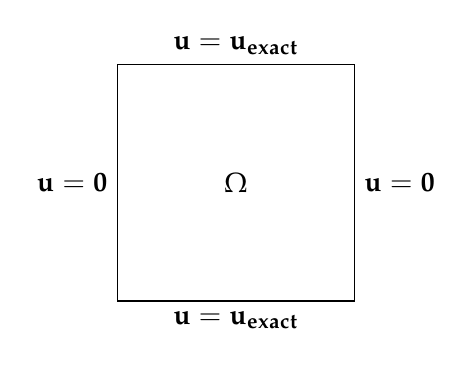
\begin{tikzpicture}
\node[
      draw,
      minimum height=3cm,
      minimum width=3cm,
      label=0:$\mathbf{u=0}$,%< -- This uses angle zero degree on the border for the location
      label=west:$\mathbf{u=0}$, %< -- This uses an anchor of the node for the location
      label=north:$\mathbf{u=u_{exact}}$,
      label=south:$\mathbf{u=u_{exact}}$
] at (0,1.5) {$\Omega$};
\end{tikzpicture}
\end{center}

Let $\mathbf{u}_h$ and $p_h$ be two two approximate solutions obtained from the simulation, we now want compute the errors

\begin{itemize}
\item $|| \mathbf{u}_{exact} - \mathbf{u}_h ||_{L^2}$,
\item $ | \mathbf{u}_{exact} - \mathbf{u}_h |_{H^1}$ (seminorm),
\item $|| p_{exact} - p_h ||_{L^2} $.
\end{itemize}

in order to compare our exact solution with the manufactured one.
Using the previous exact solution, the error is 0, since the method for solving the problem is exact for polynomials, as shown below


\begin{center}
\begin{tabular}{| c | c | c | c |}
\hline
$\mathbf{N}$ & $\mathbf{|| u_{exact} - u_h ||_{L^2}}$ & $ \mathbf{ | u_{exact} - u_h |_{H^1}}$ & $  \mathbf{ || p_{exact} - p_h ||_{L^2}}$ \\
\hline
$ 4 $ & $2.7373 \times 10^{-14}$ & $3.2162 \times 10^{-13}$ &  $ 2.7373 \times 10^{-14}$ \\
\hline
$ 8$ & $1.3173  \times 10^{-12}$ & $7.5841 \times 10^{-11}$ &  $ 1.3172  \times 10^{-12}$ \\
\hline
$ 16 $ & $ 8.4791 \times 10^{-14}$ & $9.1285 \times 10^{-12}$ & $ 8.4791 \times 10^{-14}$ \\
\hline
$ 32$ & $9.0508 \times 10^{-14}$ & $1.6039 \times 10^{-11}$ &  $ 9.0580 \times 10^{-14}$ \\
\hline
$ 64$ & $6.3504 \times 10^{-13}$ & $9.5275 \times 10^{-11}$ &  $ 6.3504 \times 10^{-13}$ \\
\hline
\end{tabular}
\end{center}

\vspace{1cm}

A difference exact solution that could be used is:

\[
\mathbf{u}_{exact} = \left[ \begin{array}{c} 0 \\ sin(\pi x) \end{array} \right], \quad
p_{exact} = \frac{1}{2}-y.
\]

%(Reminder: I put the $\pi$ in order for the exact solution to satisfy the boundary conditions!)
In the following tables, the convergence rate $k$ was computed, according to:

\[
k = \frac{log(\frac{E_{i+1}}{E_i})}{log(\frac{h_{i+1}}{h_i})}
\]

where we are assuming that $E_i \sim h^k_i$ and $E_{i+1} \sim h^k_{i+1}$. \\
The following table shows a second order convergence rate in $H^1$, as confirmed by the convergence plot.

\vspace{1cm}
\begin{figure}[h!]
\centering
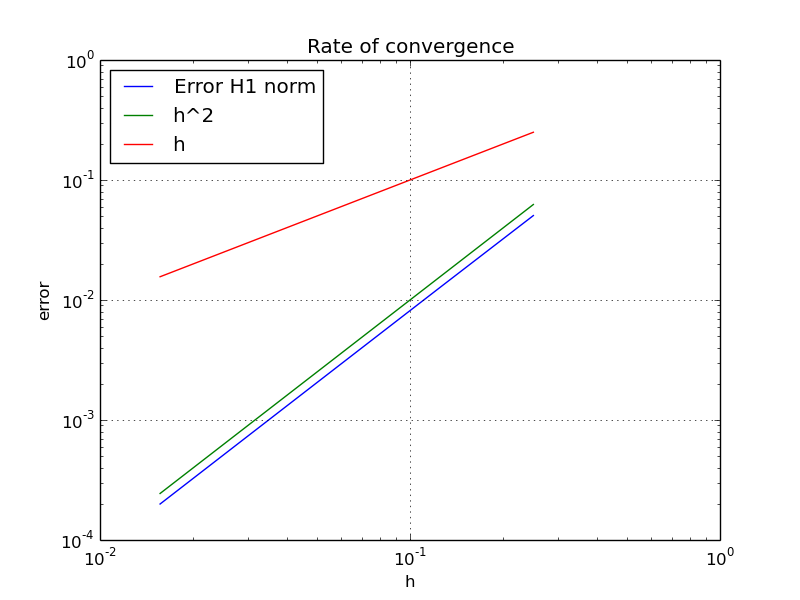
\includegraphics[width=\textwidth]{images/convergence_sine}
\caption{The plot shows a second order convergence, since the blue and green lines are parallel.}
\end{figure}
\vspace{1cm}

\begin{center}
\begin{tabular}{| c | c | c | c | c |}
\hline
$  \mathbf{N}$ & $ \mathbf{|| u_{exact} - u_h ||_{L^2}}$ & $  \mathbf{ | u_{exact} - u_h |_{H^1}}$ & \textbf{Rate in }  $ \mathbf{L^2}$ & \textbf{Rate in } $  \mathbf{H^1}$  \\
\hline
$ 4 $ & $1.9388 \times 10^{-3}$ & $5.0548 \times 10^{-2}$  & & \\
\hline
$ 8$ & $2.4515  \times 10^{-4}$ & $1.2733 \times 10^{-2}$ &  $2.9834$ &  $1.9890$   \\
\hline
$ 16 $ & $ 3.0745 \times 10^{-5}$ & $3.1896 \times 10^{-3}$ & $ 2.9952 $ & $1.9971$   \\
\hline
$ 32$ & $3.8465 \times 10^{-6}$ & $7.9780 \times 10^{-4}$ & $ 2.9987 $ & $ 1.9992 $  \\
\hline
$ 64$ & $4.8092 \times 10^{-7}$ & $1.9948 \times 10^{-4}$  & $ 2.9997 $ & $1.9998$ \\
\hline
\end{tabular}
\end{center}



\begin{center}
\begin{tabular}{| c | c | c |}
\hline
$\mathbf{N}$ & $\mathbf{|| p_{exact} - p_h ||_{L^2}}$ & \textbf{Rate in } $  \mathbf{L^2}$  \\
\hline
$ 4 $ & $1.4420  \times 10^{-4} $ & \\
\hline
$ 8 $ & $ 1.1896  \times 10^{-5} $ & $3.5995$ \\
\hline
$ 16 $ & $ 1.0089  \times 10^{-6} $ & $3.5596$ \\
\hline
$ 32 $ & $  8.7143 \times 10^{-8} $ & $3.5332$ \\
\hline
$ 64 $ & $ 8.0070 \times 10^{-9} $ & $3.4440$ \\
\hline
\end{tabular}
\end{center}


\subsection{MMS for Navier-Stokes equations with parabolic inlet velocity}
\label{parabolic inlet}
We now want to verify our Navier-Stokes solver using MMS. We start from Navier-Stokes equations written in the form (\ref{eq:ns:3}), with $\mu = 1/8$.  Let $\Omega$ be the unit square $\Omega = [0,1]^2$. We want to solve the N-S equation in the domain $\Omega$ applying the following boundary conditions:

\begin{center}
\begin{tikzpicture}
\node[
      draw,
      minimum height=3cm,
      minimum width=3cm,
      label=0:$\sigma \cdot \mathbf{n}$ \text{=}$ -p_{out} \mathbf{n}$,%< -- This uses angle zero degree on the border for the location
      label=west:$\sigma \cdot \mathbf{n}$ \text{=}$ -p_{in} \mathbf{n}$, %< -- This uses an anchor of the node for the location
      label=north:$\mathbf{u=0}$,
      label=south:$\mathbf{u=0}$
] at (0,1.5) {$\Omega$};
\end{tikzpicture}
\end{center}

i.e. $\mathbf{u=0}$ on the top and bottom boundaries, and we apply a pressure difference on the sides, so the fluid can move from left to right. The exact solution for this problem is $\mathbf{u}(y) = [\frac{1}{2\mu} y (1-y), 0]$ and $p(x) = 1-x$. Comparing the numerical solution from our solver with the exact solution, the error is 0:

\begin{center}
\begin{tabular}{| c | c | c | c | c |}
\hline
$\mathbf{N}$ & $\mathbf{dt (= \frac{1}{N})}$ & $\mathbf{|| u_{exact} - u_h ||_{L^2}}$ & $ \mathbf{ | u_{exact} - u_h |_{H^1}}$ & $  \mathbf{ || p_{exact} - p_h ||_{L^2}}$ \\
\hline
$ 4 $ & $ 0.25 $ & $2.5488 \times 10^{-10}$ & $8.0081 \times 10^{-10}$ &  $ 3.7574 \times 10^{-13}$ \\
\hline
$ 8$ & $ 0.125 $ & $6.8121  \times 10^{-11}$ & $2.1401 \times 10^{-10}$ &  $ 1.3412  \times 10^{-14}$ \\
\hline
$ 16 $ & $ 0.0625 $ & $ 3.1065 \times 10^{-11}$ & $9.7595 \times 10^{-11}$ & $ 9.0360 \times 10^{-15}$ \\
\hline
$ 32$ & $ 0.03125 $ & $1.6841 \times 10^{-11}$ & $5.2914 \times 10^{-11}$ &  $ 1.5517 \times 10^{-14}$ \\
\hline
$ 64$ & $ 0.015625 $ & $1.2541 \times 10^{-12}$ & $1.6649 \times 10^{-11}$ &  $ 3.5736 \times 10^{-13}$ \\
\hline
\end{tabular}
\end{center}

\begin{figure}[ht]
\centering
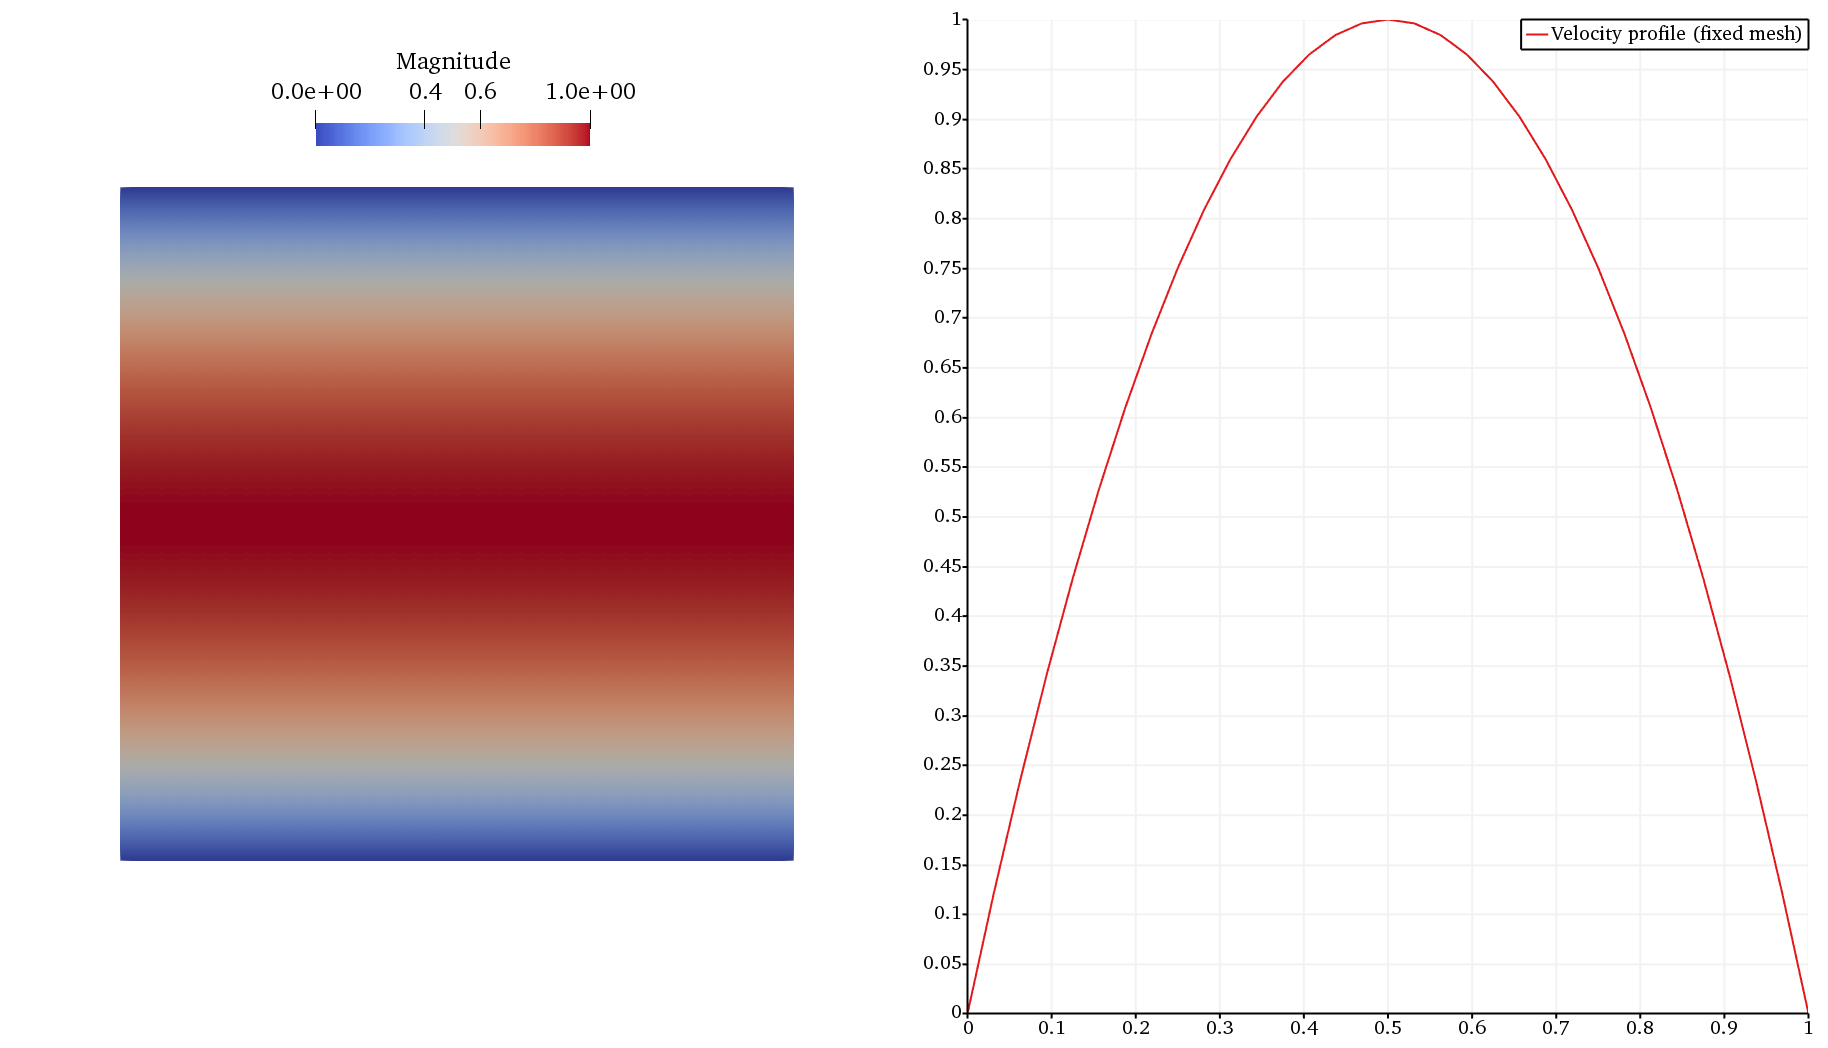
\includegraphics[width=\textwidth]{images/velocity_fixed.png}
\caption{caption}
\end{figure}

\subsection{Pressure-driven channel flow (2D)}
% References:
% Fenics book
% http://faculty.kfupm.edu.sa/CHE/usamah/CHE204/CHE204-HD22%20-%20Flow%20Through%20Circular%20Pipe.pdf

% Should I add some theory on this?

A typical test problem is finding the solution of the Navier-Stokes equations in a two-dimensional pressure-driven channel. We consider a viscous flow between parallel plates, where the geometry is the unit square $[0,1]^2$, and the kinematic viscosity is $\nu = 1/8$. We assume that both plates are fixed, i.e. no-slip boundary conditions are applied to the velocity at the upper and lower walls, and Neumann boundary conditions $\sigma \cdot \vec{n} = 0$ are applied at the inlet and outlet. Dirichlet boundary conditions are applied to the pressure at the inlet and outlet, with $p = 1$ at the inlet and $p = 0$ at the outlet. The initial condition for the velocity is $\mathbf{u} = (0,0)$. As a reference value in order to verify the agreement of our solution, we use the $x$-component of the velocity at the point $(x, y) = (1, 0.5)$ at final time $T = 0.5 $. The value reported on the FEniCS book [PUT REFERENCE] is $u_x(1, 0.5, T=0.5) \approx 0.44321183655681595$, while the one obtained in our results is $0.443217320106$.

\begin{figure}[h!]
\centering
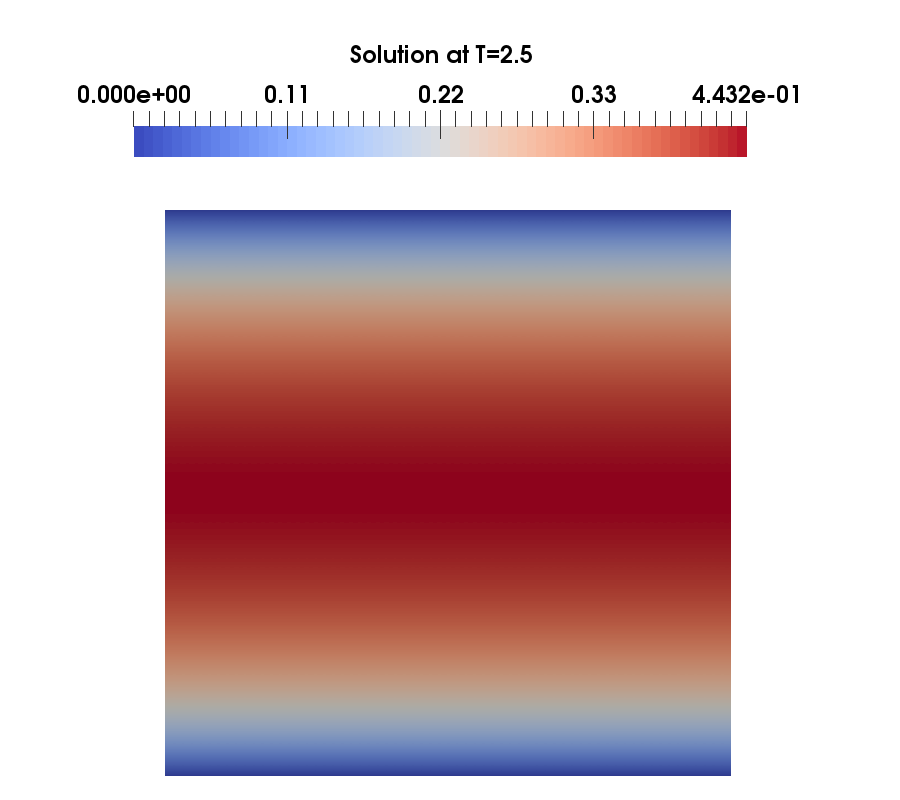
\includegraphics[width=0.8\textwidth]{images/velocity_solution.png}
\caption{Pressure driven channel flow. The plot shows the solution $u(x,y)$ for $\nu = 1/8$.}
\end{figure}

\begin{figure}[h!]
\centering
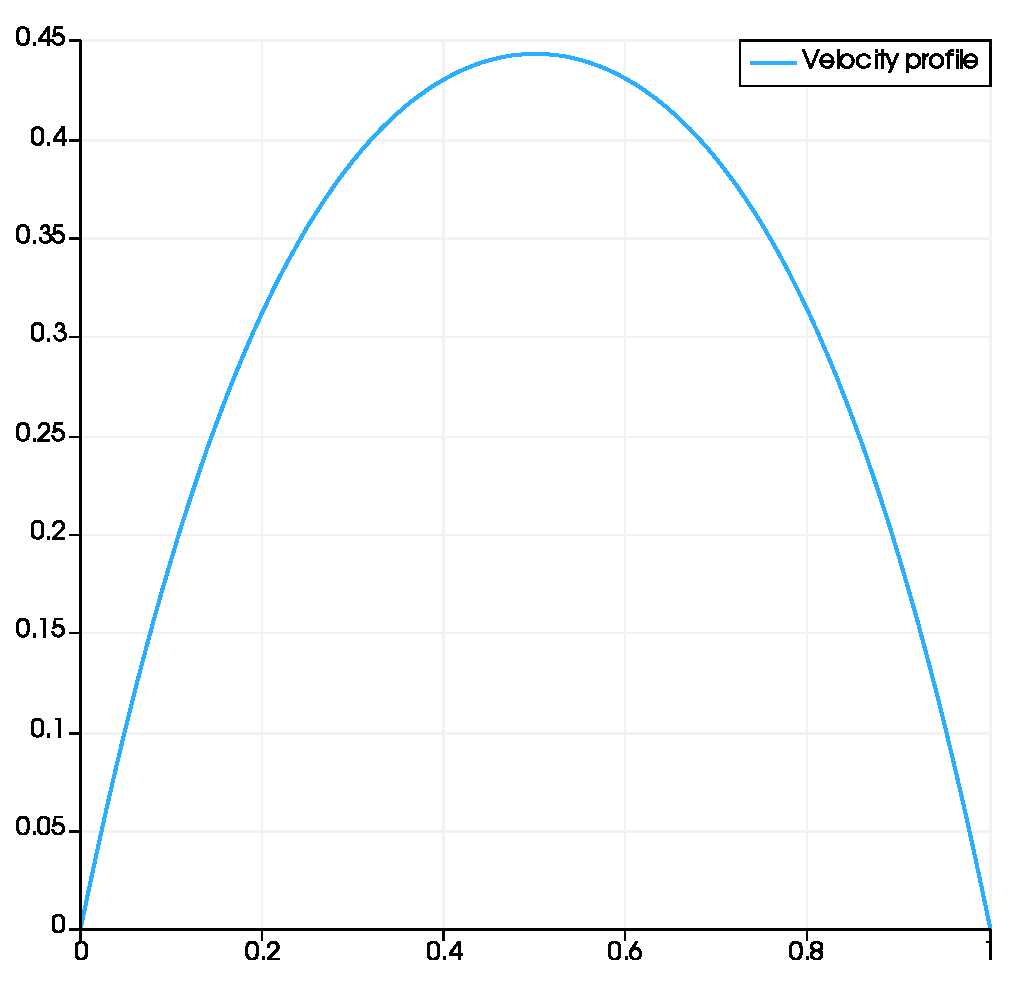
\includegraphics[width=0.6\textwidth]{images/velocity_profile.pdf}
\caption{Pressure driven channel flow. Velocity profile at the points $(0.5, 1)$ and $(0.5, 0)$.}
\end{figure}

\subsection{Driven cavity}
% References:
% Fenics book, Quarteroni, Fluid dynamics F. White

A typical benchmark problem for fluid flow solvers in the two-dimensional lid-driven cavity problem. We consider a square cavity $\Omega$ with sides of unit length, i.e. $\Omega = [0,1] \times [0,1]$, kinematic viscosity $\nu = 1/1000$, and density $\rho = 1$. No-slip boundary conditions are imposed on each edge of the square, except at the upper edge where the velocity is set to $\mathbf{u} = (1,0)^T$, as follows

\[
\begin{cases}
\mathbf{u} = (0, 0)^T, & \mbox{on } \partial \Omega \backslash \Gamma \\
\mathbf{u} = (1, 0)^T, & \mbox{on } \Gamma
\end{cases}
\]

where $ \Gamma = \set{ \mathbf{x} = (x,y)^T \in \partial \Omega | y = 1}$. We use finite elements on triangular grids of the type $\mathcal{P}_2-\mathcal{P}_1$. The initial condition for the velocity is set to zero. The resulting flow is a vortex developing in the upper right corner and then traveling towards the center of the square as the flow evolves. \\
To verify the correctness of the solver, we consider the minimum of the \textit{stream function}. The stream function $\psi$ allows us to satisfy the continuity equation and then solve the momentum equation directly for the single variable $\psi$. It is defined by

\[
\mathbf{u} = \nabla \times \psi = (\frac{\partial \psi}{\partial y} , - \frac{\partial \psi }{\partial x}),
\]

and it can be computed by solving the Poisson problem

\[
- \nabla^2 \psi = \omega,
\]

where $\omega$ is the vorticity given by

\[
\omega = \nabla \times \mathbf{u} = \frac{\partial u_y}{\partial x} - \frac{\partial u_x}{\partial y}.
\]


As a reference value, we use the one reported on the FEniCS book [REFERENCE], where the solution at the final time $T = 2.5$ was computed using the spectral element code Semtex with up to $80 \times 80$ $10^{th}$ order elements, heavily refined in the area in the vicinity of the minimum of the stream function. The time-stepping for computing the reference solution was handled by a third order implicit discretization, and a very short time step was used to minimize temporal errors.  The obtained reference value was $min(\psi) = -0.061 077$.

\begin{figure}[ht]
\centering
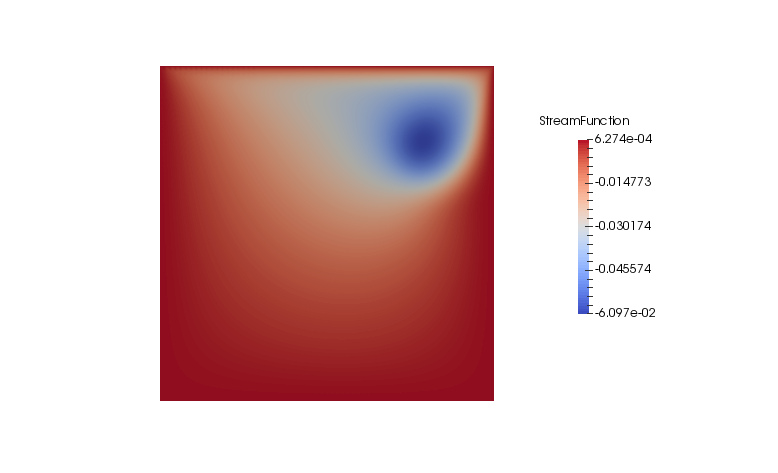
\includegraphics[width=\textwidth]{images/oyvind.png}
\vspace{-1cm}
\caption{Driven cavity. The plot shows the stream function, and its minimum value $-0.06097$. This reference solution is taken from an already validated code (reference to OASIS).}
\end{figure}


In our case, a Crank-Nicolson (second order) discretization was used, with $\theta = 0.5$. A $64 \times 64$ number of elements was used, with $dt = 0.0125$ as time step. Hence, the obtained value was $min(\psi) = -0.061 121$, in fair agreement with the reference one. \\

\vspace{-.3cm}
\begin{figure}[ht]
\centering
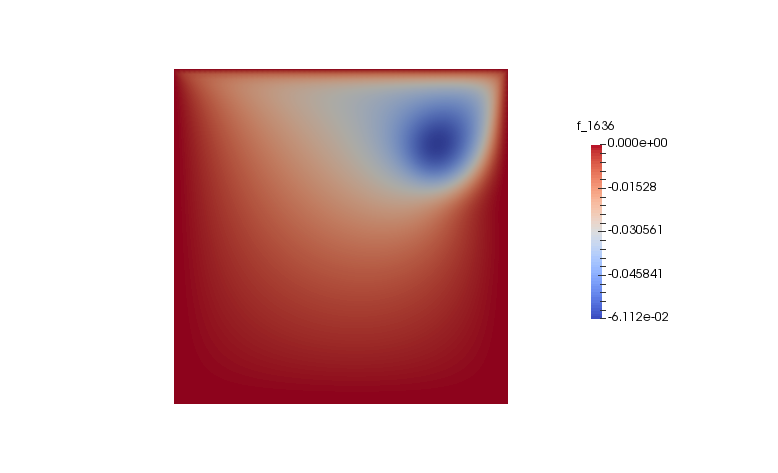
\includegraphics[width=\textwidth]{images/mine.png}
\vspace{-1cm}
\caption{Driven cavity. The plot shows the stream function, and its minimum value $-0.061 121$.}
\end{figure}


\subsection{Nitsche's method}
Now we want to use the Nitsche method to the driven cavity test case, in order to apply Dirichlet boundary conditions in a weak way. We consider a square cavity $\Omega$ with sides of unit length, i.e. $\Omega = [0,1] \times [0,1]$, kinematic viscosity $\nu = 1/1000$, and density $\rho = 1$. No-slip boundary conditions are imposed on left and bottom edges of the square, except at the upper edge where the velocity is set to $\mathbf{u} = (1,0)^T$, as follows

\[
\begin{cases}
\mathbf{u} = (0, 0)^T, & \mbox{on } \partial \Omega \backslash (\Gamma_1 \cup \Gamma_2) \\
\mathbf{u} = (1, 0)^T, & \mbox{on } \Gamma_1
\end{cases}
\]

where $ \Gamma_1 = \set{ (x,y)^T \in \partial \Omega | y = 1}$ and
$ \Gamma_2 = \set{ (x,y)^T \in \partial \Omega | x = 1}$. On the boundary $\Gamma_2$ we will apply the condition $\mathbf{u} = \mathbf{g} = (0,0)^T$ in a weakly way using Nitsche's method. Substituting (\ref{eq:green}) in (\ref{eq:ns:9}) we have

\begin{align}
\int_{\Omega} \rho \dot{\mathbf{u}} \, \mathbf{v} \, dx
+ \int_{\Omega} \rho \nabla \mathbf{u} \cdot (\mathbf{u} - \mathbf{w}) \, \mathbf{v} \, dx
+ \int_{\Omega} (\mu \nabla \mathbf{u} - pI) \cdot \nabla \mathbf{v} \, dx \\
- \int_{\partial \Omega} (\mu \nabla \mathbf{u} - pI) \cdot \mathbf{n} \, \mathbf{v} \, ds.
= \int_{\Omega} \mathbf{f} \mathbf{v} \, dx.
\end{align}

Since we are applying Dirichlet boundary conditions on $\partial \Omega \backslash \Gamma_2$, $\mathbf{v} = (0,0)$, hence 

\begin{align}
\int_{\Omega} \rho \dot{\mathbf{u}} \, \mathbf{v} \, dx
+ \int_{\Omega} \rho \nabla \mathbf{u} \cdot (\mathbf{u} - \mathbf{w}) \, \mathbf{v} \, dx
+ \int_{\Omega} (\mu \nabla \mathbf{u} - pI) \cdot \nabla \mathbf{v} \, dx \\
- \int_{\Gamma_2} (\mu \nabla \mathbf{u} - pI) \cdot \mathbf{n} \, \mathbf{v} \, ds.
= \int_{\Omega} \mathbf{f} \mathbf{v} \, dx.
\end{align}

and from (\ref{eq:bc:5}), the latter can be written as

\begin{align}
\int_{\Omega} \rho \dot{\mathbf{u}} \, \mathbf{v} \, dx
+ \int_{\Omega} \rho \nabla \mathbf{u} \cdot (\mathbf{u} - \mathbf{w}) \, \mathbf{v} \, dx
+ \int_{\Omega} (\mu \nabla \mathbf{u} - pI) \cdot \nabla \mathbf{v} \, dx \\
- \int_{\Gamma_2} (\mu \frac{\partial \mathbf{u}}{\partial \mathbf{n}} -  p \mathbf{n}) \, \mathbf{v} \, ds
= \int_{\Omega} \mathbf{f} \mathbf{v} \, dx.
\end{align}

We now apply the Nitsche method on the boundary term $\Gamma_2$, that leads to

\begin{align}
\int_{\Omega} \rho \dot{\mathbf{u}} \, \mathbf{v} \, dx
+ \int_{\Omega} \rho \nabla \mathbf{u} \cdot (\mathbf{u} - \mathbf{w}) \, \mathbf{v} \, dx
+ \int_{\Omega} (\mu \nabla \mathbf{u} - pI) \cdot \nabla \mathbf{v} \, dx \\
- \int_{\Gamma_2} \mu \frac{\partial \mathbf{u}}{\partial \mathbf{n}} \, \mathbf{v} \, ds
- \int_{\Gamma_2} \mu \frac{\partial \mathbf{v}}{\partial \mathbf{n}}  \, \mathbf{u} \, ds
+ \frac{\gamma}{h} \int_{\Gamma_2} \mathbf{u \, v} ds \\
= - \int_{\Gamma_2} \mu \frac{\partial \mathbf{v}}{\partial \mathbf{n}}  \, \mathbf{g} \, ds
+ \frac{\gamma}{h} \int_{\Gamma_2} \mathbf{g \, v} ds
+  \int_{\Omega} \mathbf{f} \mathbf{v} \, dx.
\end{align}

A $128 \times 128$ number of elements was used with $dt = 0.0125$ as time step. The obtained value was $min(\psi) = -0.0597826179273$. 

\begin{figure}[ht]
\centering
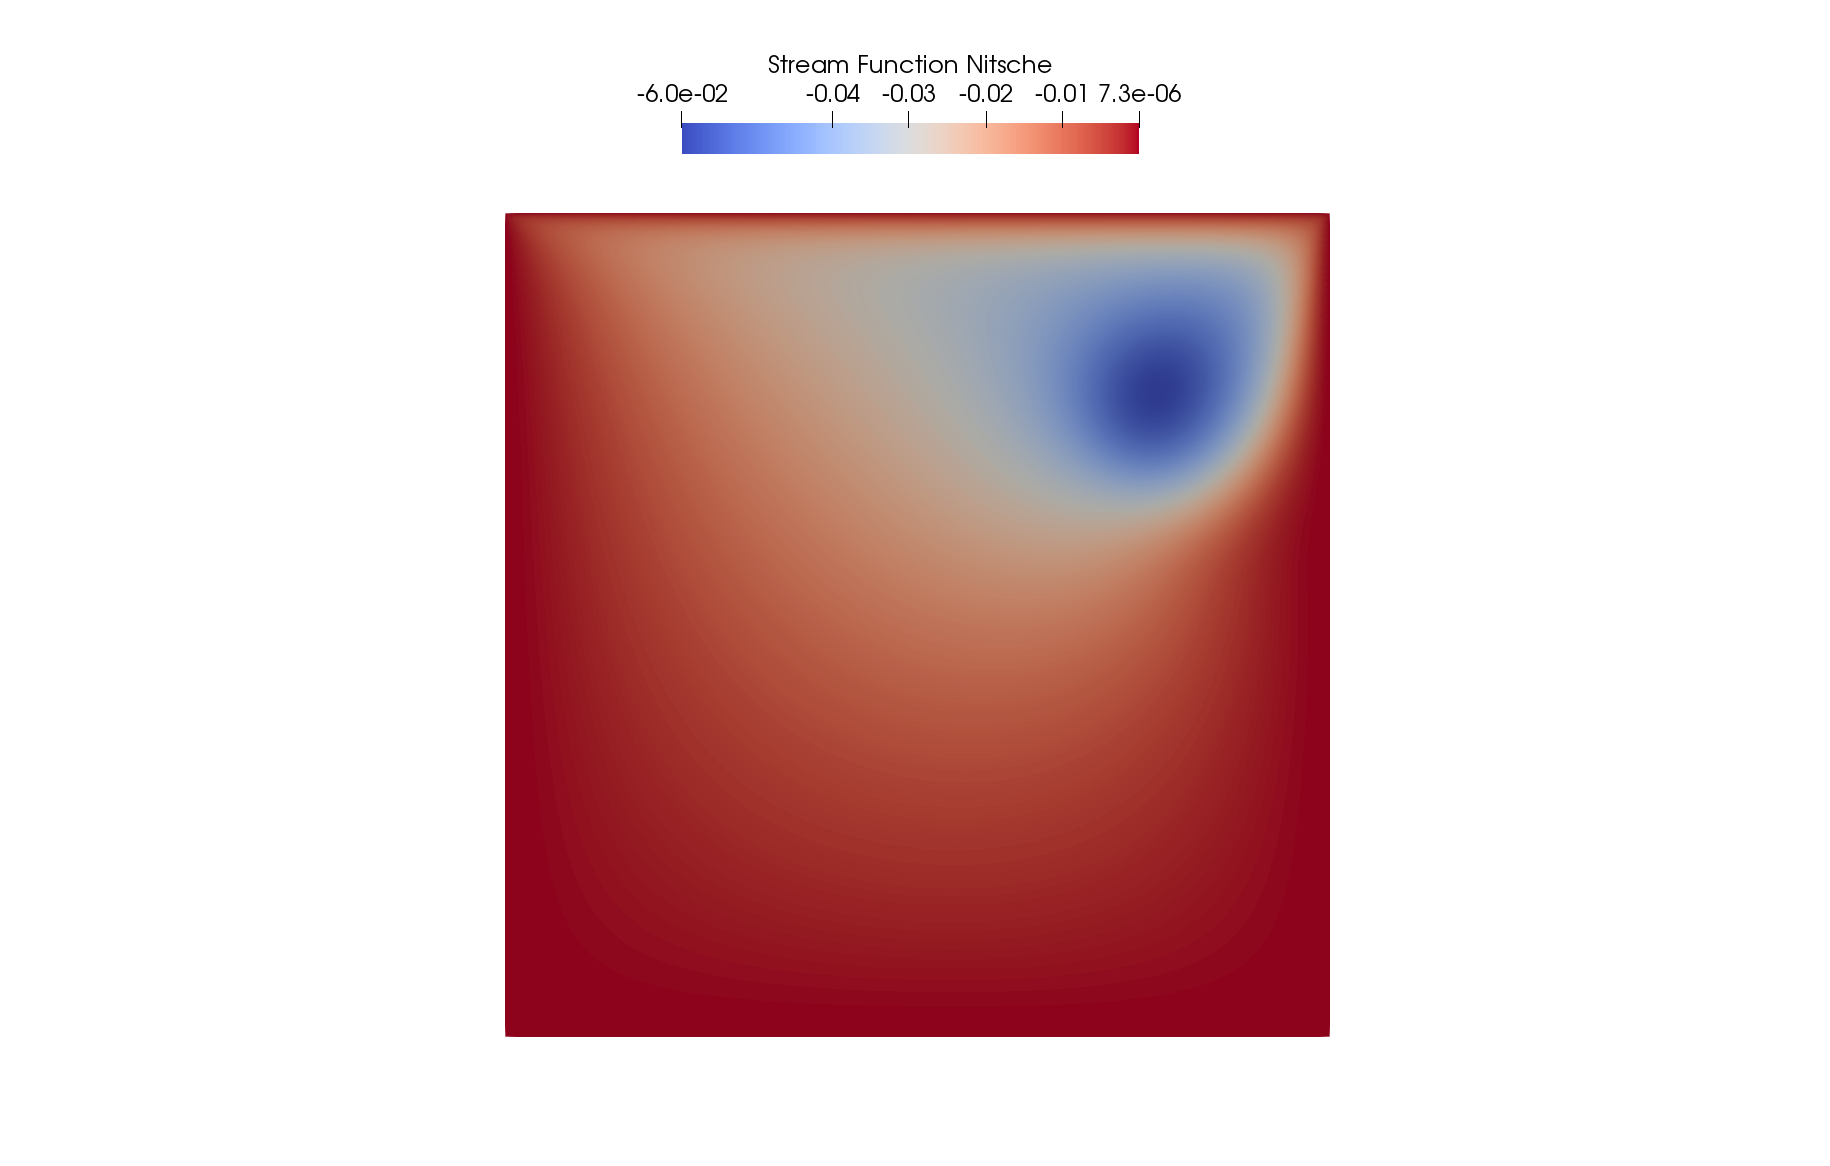
\includegraphics[width=\textwidth]{images/stream_function_nitsche.png}
\vspace{-1cm}
\caption{Driven cavity with Nitsche. The plot shows the stream function, and its minimum value $-0.05978$.}
\end{figure}

\newpage

\section{Navier-Stokes equations on a moving mesh}
\subsection{Parabolic inlet velocity with fixed mesh motion}
In this section we add a fixed mesh motion to the test case in section \ref{parabolic inlet}. We start from the NS equations with ALE term written in the form (\ref{eq:ns:1})-(\ref{eq:ns:2}) with $\mu = 1/8$. In our case, the rigid motion will be given by the vector $\mathbf{w} = [0.05, 0.05]^T$. The solution is qualitatively the same as in section \ref{parabolic inlet}, as shown by the following plot, where we plotted the velocity profile between the points $(0.5, 0)$ and $(0.5, 1)$.

\begin{figure}[ht]
\centering
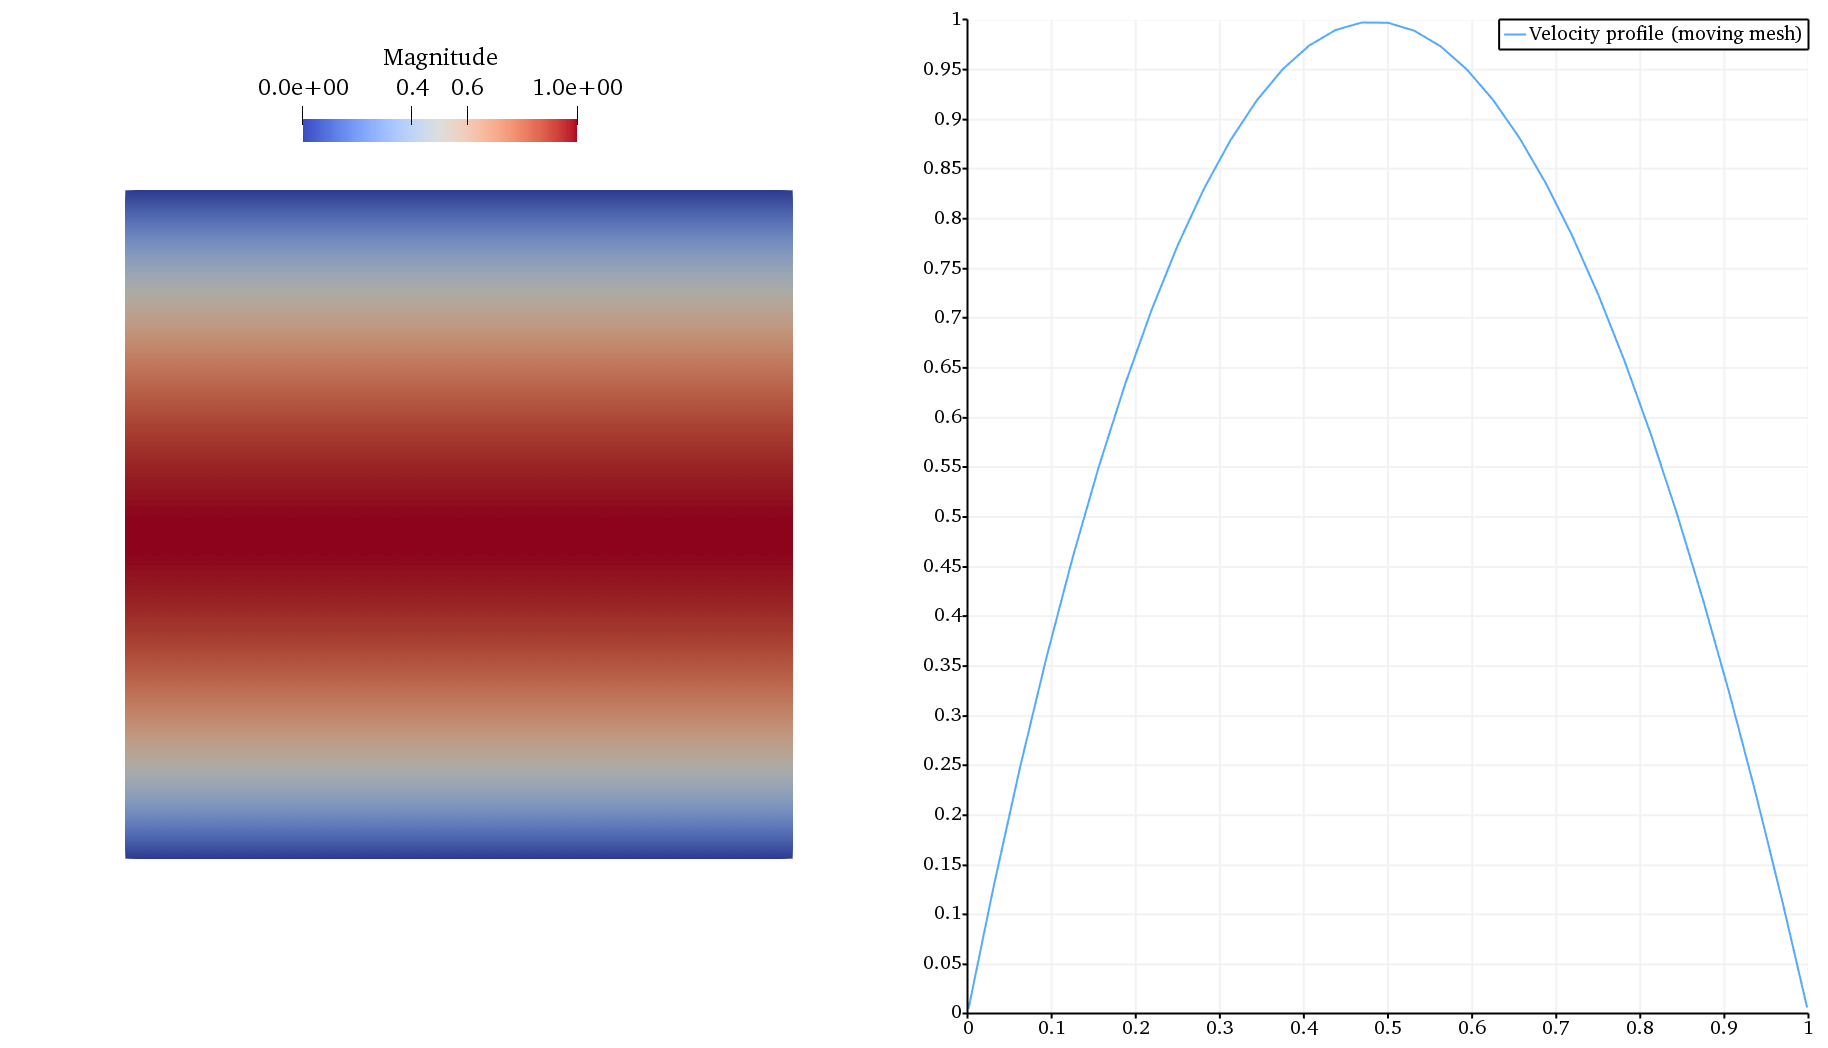
\includegraphics[width=\textwidth]{images/velocity_moving.png}
\caption{caption}
\end{figure}

\chapter{SAS simulations}

\chapter{Conclusions}

\end{document}
